% ---------------------------------------------------------------------------
% Author guideline and sample document for EG publication using LaTeX2e input
% D.Fellner, v1.20, Jan 18, 2023

\documentclass{egpubl}
\usepackage{egsr2025_DLOnlyTrack}
\title{Content-Aware Texturing for Gaussian Splatting}
% for anonymous conference submission please enter your SUBMISSION ID
% instead of the author's name (and leave the affiliation blank) !!
% for final version: please provide your *own* ORCID in the brackets following \orcid; see https://orcid.org/ for more details.
\author[Panagiotis Papantonakis \& Georgios Kopanas \& Frédo Durand \& George Drettakis]
{\parbox{\textwidth}{\centering Panagiotis Papantonakis$^{1,2}$\orcid{0009-0009-5058-1249},
        Georgios Kopanas\thanks{work done at Google}$^{3,4}$\orcid{0009-0002-5829-2192},
        Frédo Durand$^{5}$\orcid{0000-0001-9919-069X}
        and George Drettakis$^{1,2}$\orcid{0000-0002-9254-4819}
}\\
{\parbox{\textwidth}{\centering $^1$ Inria $^2$ Université Côte D'Azur $^3$ Google $^4$ Runway ML
         $^5$MIT CSAIL
       }
   }
}
% \author[Panagiotis Papantonakis]{Panagiotis Papantonakis}

% --- for  Annual CONFERENCE
% \ConferenceSubmission   % uncomment for Conference submission
% \ConferencePaper        % uncomment for (final) Conference Paper
% \STAR                   % uncomment for STAR contribution
% \Tutorial               % uncomment for Tutorial contribution
% \ShortPresentation      % uncomment for (final) Short Conference Presentation
% \Areas                  % uncomment for Areas contribution
% \Education              % uncomment for Education contribution
% \Poster                 % uncomment for Poster contribution
% \DC                     % uncomment for Doctoral Consortium
%
% --- for  CGF Journal
% \JournalSubmission    % uncomment for submission to Computer Graphics Forum
% \JournalPaper         % uncomment for final version of Journal Paper
%
% --- for  CGF Journal: special issue
% \SpecialIssueSubmission    % uncomment for submission to , special issue
\SpecialIssuePaper         % uncomment for final version of Computer Graphics Forum, special issue
%                          % EuroVis, SGP, Rendering, PG
% --- for  EG Workshop Proceedings
% \WsSubmission      % uncomment for submission to EG Workshop
\WsPaper           % uncomment for final version of EG Workshop contribution
% \WsSubmissionJoint % for joint events, for example ICAT-EGVE
% \WsPaperJoint      % for joint events, for example ICAT-EGVE
% \Expressive        % for SBIM, CAe, NPAR
% \DigitalHeritagePaper
% \PaperL2P          % for events EG only asks for License to Publish

% --- for EuroVis 
% for full papers use \SpecialIssuePaper
% \STAREurovis   % for EuroVis additional material 
% \EuroVisPoster % for EuroVis additional material 
% \EuroVisShort  % for EuroVis additional material
% \MedicalPrize  % uncomment for Medical Prize (Dirk Bartz) contribution, since 2021 part of EuroVis

% Licences: for CGF Journal (EG conf. full papers and STARs, EuroVis conf. full papers and STARs, SR, SGP, PG)
% please choose the correct license
%\CGFStandardLicense
\CGFccby
%\CGFccbync
%\CGFccbyncnd

% !! *please* don't change anything above
% !! unless you REALLY know what you are doing
% ------------------------------------------------------------------------
\usepackage[T1]{fontenc}
\usepackage{dfadobe}  

%\usepackage{cite}  % comment out for biblatex with backend=biber 
% ---------------------------
\biberVersion
\BibtexOrBiblatex
\usepackage[backend=biber,bibstyle=EG,citestyle=alphabetic,backref=true]{biblatex} 
\addbibresource{references.bib}
% ---------------------------  
\electronicVersion
\PrintedOrElectronic

% for including postscript figures
% mind: package option 'draft' will replace PS figure by a filename within a frame
\ifpdf \usepackage[pdftex]{graphicx} \pdfcompresslevel=9
\else \usepackage[dvips]{graphicx} \fi

\usepackage{egweblnk} 
% end of prologue
\usepackage{amssymb, amsmath}
\usepackage{booktabs}
\usepackage{multirow}
\usepackage[table]{xcolor}
\usepackage{tabularx}
\usepackage{graphicx}
\usepackage{tikz}
\usetikzlibrary{spy}
\usepackage{rotating}
\usepackage{soul}

\usepackage[ruled]{algorithm2e}

\begin{document}
% uncomment for using teaser
\teaser{
 \includegraphics[width=1\linewidth]{images/teaser_split_texture_onoff_new.pdf}
\centering
\caption{
We propose a content-aware texturing method for 2D Gaussian Splatting.  Our textures reconstruct intricate scene detail (a). Gaussian primitives reconstruct the shape of the scene at low frequency of appearance; we show this in (b) where texturing is disabled. Our method is adaptive, allowing different primitives to have different texel sizes, depending on scene content. On the right hand panel we display primitives with progressively higher \emph{texel-to-pixel} ratio. In regions with high frequency appearance, texels have size close that of pixels (e.g., the table cover (c)). For the low-frequency walls however (d), the ratio is high, with each texel representing a large number of input image pixels.
%By iteratively adjusting the texel size,
%our textures match the frequency content of the scene(right).
% Guided by the scene's content and how well the textures represent it,
% their ratios get iteratively updated.
% Our method achieves competitive results while requiring fewer parameters than other texturing methods.
}
\label{fig:teaser}
}

\newcommand{\missingcitation}[1]{\textcolor{magenta}{#1}}
\newcommand{\TODO}[1]{}
% \newcommand{\TODO}[1]{\textcolor{red}{#1}}
\newcommand{\PP}[1]{\textcolor{cyan}{#1}}
\newcommand{\GD}[1]{\textcolor{blue}{#1}}
\newcommand{\GK}[1]{\textcolor{brown}{#1}}
\newcommand{\Fredo}[1]{\textcolor{orange}{Fr\'edo: #1}}
% \newcommand{\revision}[2]{\textcolor{red}{#2}}
\newcommand{\revision}[2]{#2}
\definecolor{tabfirst}{rgb}{1, 0.7, 0.7} % red

\definecolor{tabsecond}{rgb}{1, 0.85, 0.7} % orange
\definecolor{tabthird}{rgb}{1, 1, 0.7} % yellow

\newcommand{\mvec}[1]{\mathbf{#1}}

\newcommand{\spyimage}[5]{%
	\begin{tikzpicture}[spy using outlines={rectangle,#1,magnification=5,size=1cm, connect spies}]
		\node[anchor=south west,inner sep=0]  at (0,0) {\includegraphics[width=#2]{#3}};
		\spy on (#4) in node [left] at (#5);
	\end{tikzpicture}%
}

\maketitle
\begin{abstract}
Gaussian Splatting has become the method of choice for 3D reconstruction and real-time rendering of captured real scenes.
However, fine appearance details  need to be represented as a large number of small Gaussian primitives, which can be wasteful when geometry and appearance exhibit different frequency characteristics.
Inspired by the long tradition of texture mapping, we propose to use texture to represent detailed appearance where possible.
Our main focus is to incorporate per-primitive texture maps that adapt to the 
%\emph{content} of the 
scene in a principled manner during Gaussian Splatting optimization.
We do this by proposing a new appearance representation for 2D Gaussian primitives with textures where the size of a texel is bounded by the image sampling frequency and adapted to the content of the input images. 
We achieve this by adaptively upscaling or downscaling the texture resolution during optimization.
In addition,
our approach enables control of the number of primitives during optimization based on texture resolution.
We show that our approach performs favorably in image quality and  total number of parameters used compared to alternative solutions for textured Gaussian primitives.
\end{abstract}

\section{Introduction}
%
%\GD{Following is just to help me structure my thoughts}
%\begin{itemize}
%\item 3DGS and variants use a mixture of splats and SH's to represent appearance
%\item Texture is a compact and effective way of representing high frequency
%appearance attached to a surface
%\item Total number of parameters of the representation: Primitives, with position (mean), scale, rotation for shape together with opacity and SH for appearance; and texture resolution.
%\item We strive to exploit compact texture as much as possible; this requires a choice of how to distribute the parameter burden between the primitives and the texture in a principled manner.
%\item We introduce a principled approach to resolution and primitive management, based on the content in the input images, by setting world-space texel size based on available resolution in the input.
%\end{itemize}
%
%\TODO{Standard Intro}

Gaussian Splatting~\cite{3dgs,2dgs} has become the method of choice for the  capture and real-time novel-view synthesis of real scenes. It relies on flexible, easy-to-optimize \emph{Gaussian primitives} to represent the scene.
However, in the standard approach, fine visual appearance -- such as intricate texture on a surface -- needs to be represented with a large number of very small primitives even when the geometric complexity is low. 
This wasteful limitation arises because each Gaussian primitive is associated with a single color sample, preventing the decoupling of appearance and geometric complexity.
Rendering techniques, on the other hand, have traditionally built on \emph{texture mapping} to represent such detailed appearance. We build on this tradition to propose a representation for {\em textured} Gaussian primitives that is guided by the scene and its content.

In recent and concurrent work~\cite{bbsplat, gstex, textured3dgs, supergaussians} a number of methods introduce textured Gaussian primitives, 
providing a spatially varying color.
Most of these methods
use planar 2D Gaussians to match the dimensionality of traditional textures.
Each primitive carries several parameters (position, rotation, scale, opacity and spherical harmonics (SH)),
while textures are 2D arrays of RGB(A) texels.
The fundamental challenge of such approaches is how to allocate model capacity across the scene
and between the number of texels and the number of primitives used.
Previous and concurrent solutions either deal with the issue by imposing a fixed texture resolution per primitive~\cite{bbsplat, supergaussians, textured3dgs}, or propose heuristic approaches, that are far from ideal~\cite{gstex}.
This leaves open the question of how to share resources in a more principled manner.%between texels and primitives.

To answer this question,
we propose a \emph{content-aware} texturing solution for 2D Gaussian primitives that uses the appearance complexity \revision{rev6315 term content unclear}{as observed from the input images of the scene} to make informed decisions on how parameter resources
are distributed.
We do this by first introducing a textured Gaussian primitive representation in which texel size is \emph{fixed} in world space.
\revision{rev6315 term content unclear}{
This makes the appearance texture of each primitive independent of its size,
and therefore unaffected by the growing or shrinking that it undergoes during optimization.
This representation separates the parameters of geometry and appearance, allowing us to refine them independently with appropriate allocation of memory capacity.
%As a result, we can develop methods that allocate model capacity to refine the two independently.
%This enables us to refine 
}
% , estimated using the content of the input images.
More specifically,
we introduce a method to increase and decrease the texel size as optimization evolves,
by analyzing the frequency content that primitive textures can represent and determining the corresponding error.
We pair that with a resolution-aware method to control the overall number of primitives,
striking a balance between texture size and number of primitives.
Our solution interacts closely with the optimization,
using the downscale/upscale mechanism to reduce the error in \emph{appearance},
while our control of the number of primitives handles \emph{geometric} error by spawning additional Gaussians to capture geometric detail.

%\begin{itemize}
%\item 3DGS is great, but requires tons of small primitives, mixing appearance and shape 
%\item Texture is great (standard CG), good representation of surface detail
%\item Several efforts to combine the two. Problem of how to assign texture resolution, usually ad-hoc
%\item We introduce a principled, content-aware approach
%\begin{itemize}
%\item Review previous methods at a high level, say heuristics
%\item Need for a principled approach rather than ad-hoc
%\end{itemize}
%
%\begin{itemize}
%\item We introduce a principled content-aware approach, 
%\item Explain representation, need for frequency content adaptation and
%progressive approach, need for splitting
%\item Contribs: 

\noindent
In summary,
we propose three contributions:
\begin{itemize}
\item A texture representation for 2D Gaussians that defines texels with a \emph{fixed} world space size, supporting visual reconstruction independent of the shape of the primitives.
% \item A content-aware texture representation for Gaussian primitives,
\item A progressive algorithm that adaptively determines texel size and allows for content-aware fitting of the scene.
\item A resolution-based solution to control the number of primitives,
adjusted to the textured representation.

\end{itemize}
Our experiments show that our method provides a good balance between visual quality and the number of parameters used for the representation, comparing favorably to other textured Gaussian primitives solutions proposed in recent and concurrent work.
\section{Related Work}

\subsection{Traditional Representations}
%Representations of appearance and geometry are widely studied in Computer Graphics (CG). Arguably, different representations offer different trade-offs between expressivity, computational efficiency, and compactness. \Fredo{This intro paragraph can be deleted.}
%In other cases different representations enable useful downstream applications like animation\cite{}, physical simulation\cite{} and editing\cite{}.

%\Fredo{Overall this section is a bit %long and can be shortened.}
%\GD{I think this is fine}

\emph{Texture Mapping} was introduced in the early days of CG~\cite{catmull1974subdivision} and is widely used to effectively map detailed appearance information onto a simpler geometric representation, such as triangles. Textures are stored as 2D image arrays with a mapping function between the 3D surface and 2D texture coordinates. Computing this 2D surface parameterization is a well-studied and difficult problem~\cite{hormann2007mesh, li2018optcuts, srinivasan2024nuvo}. Intrinsic 2D parameterizations pose challenges even in traditional graphics pippelines~\cite{yuksel2019rethinking} because they introduce difficulties in content creation and produce visual artifacts in rendering. In the context of optimization for inverse problems -- such as novel view synthesis -- intrinsic parameterizations are also challenging since the geometry is not known in advance~\cite{srinivasan2024nuvo}. An alternative, non-parametric way to store localized information on the surface is by attaching it on the primitives themselves, i.e.,  attaching colors to the vertices of a mesh, requiring a very fine mesh subdivision to represent details. Mesh Colors~\cite{yuksel2010mesh,mallett2020patch} extend this idea by using more color samples along the edges and the faces of the triangles. This significantly improves the representational capacity of non-parametric appearance textures. While non-parametric appearance models are limited in many ways, they have significant advantages in the context of optimization since they overcome the need to jointly solve for texture parameterization and the surface. Our representation is also a non-parametric texture representation for Gaussian Splatting.

\subsection{Representations for 3D Reconstruction}
\label{sec:reps}
%\Fredo{Maybe skip directly to Gaussians?}\GD{Again, ok for me}\GK{My motivation to add MPI is because its a "textured" representation, kind of, happy to skip some if Fredo insists!}
Scene reconstruction and novel view synthesis has recently utilized differentiable rendering to recover 3D representations from a set of images or video. Early methods utilized Multi-Plane Images (MPIs)~\cite{mildenhall2019local,zhou2018stereo}, a collection of planes with RGBA textures that are re-projected and rendered very efficiently using homography transformations. The semi-transparent and planar nature of the RGBA textures allowed the optimization to converge to useful 3D representations, but the planar assumption for the geometry is insufficient in most realistic cases. Neural Radiance Fields (NeRF~\cite{nerf}) popularized volumetric representations in the context of 3D reconstruction by introducing an Multi-Layer Perceptron (MLP) that stores volume density and color. NeRF's success resulted in follow-up work that extended it to support anti-aliasing and unbounded scenes~\cite{mipnerf, mipnerf360, zhang2020nerf++}, improve its training and rendering speed~\cite{kilonerf, dvxgo, instant-ngp, tensorf, plenoxels, zipnerf, adaptiveshells, sharma2024volumetric}, increase its robustness when using fewer views \cite{pixelnerf, regnerf}, and better reconstruct surfaces and handle reflections~\cite{refnerf, neuralangelo, bakedsdf}. Most closely related to our work is Nuvo~\cite{srinivasan2024nuvo} that recovers a 2D parameterization of a volume. For a more complete survey we refer readers to~\cite{tewari2022advances}.

Gaussian Splatting~\cite{3dgs} has emerged as an alternative, point-based approach to NeRFs by replacing the volumetric field with a collection of semi-transparent ellipsoidal primitives. This technique achieves excellent quality and real-time rendering even at high resolutions.
Several methods built on top of 3DGS to provide anti-aliasing \cite{mipsplatting},
by changing the appearance model but are constrained by the 1-to-1 relationship between color samples and primitives~\cite{specgaussian,malarz2025gaussian}. 

2D Gaussian Splatting~\cite{2dgs} flattens one of the dimensions of the ellipsoids to create planar discs or \emph{surfels} to align better with surfaces. 
%\subsection{Preliminaries: 2D Gaussian Splatting}
%2D Gaussian Splatting \cite{2dgs},
%aimed to improve the original 3DGS method in terms of the geometrical reconstruction of scenes.
%Almost identically to 3DGS,
Surfels are parametrized by the set of parameters $A=\{\boldsymbol{\mu}, \boldsymbol {\sigma}, \mvec{q}, o, \mvec{SH}\}$,
where $\boldsymbol{\mu} \in \mathbb{R}^3$ is the primitive's center,
$\boldsymbol{\sigma} \in \mathbb{R^+}^2$ are the scales of the primal axes of the surfel,
$\mvec{q} \in \mathbb{R}^4$ is a quaternion that represents the rotation $\mvec{R}$,
$o$ is the opacity and
$\mvec{SH}$ are the spherical harmonics coefficients used to get the view-dependent colour $\mvec{c}$.
The normal vector $\mvec{n}$ of the surfel is the third column of the rotation matrix $\mvec{R}$.

With this formulation, the intersection point between a ray $\mvec{r} = \mvec{r_0} + t\mvec{d}$ and a primitive can be computed as:
\begin{equation}\label{eq:intersection_point}
\mvec{p} = \mvec{r}_0 + t\mvec{d}, t = \frac{\mvec{n} \cdot (\mvec{\mu} - \mvec{r}_0)}{\mvec{n} \cdot \mvec{d}}
\end{equation}
We also build on 2D Gaussian Splatting for our method.

The initial primitive-based representations were not as compact as NeRFs, but a number of recent results allow competitive compression strategies~\cite{3dgszip}. Several recent methods build on traditional CG solutions, demonstrating that disentangling appearance from geometry can achieve significant improvements in terms of storage and memory costs.  Texture-GS~\cite{uv3dgs} combines deferred shading and a per-pixel UV coordinate to fetch appearance from a texture. This assumes that the objects can be represented by a sphere imposing topological constraints. Our results demonstrate that non-parametric texture mapping is a convenient and flexible way to recover texture during the optimization. 

Recent and concurrent work \cite{bbsplat, textured3dgs, supergaussians, gstex} have used textures to represent fine visual details.
\cite{gstex} and \cite{textured3dgs} use converged 2DGS and 3DGS point clouds, respectively,
as a starting point of their method, and then proceed to add and optimize texture parameters.
Several methods~\cite{bbsplat, textured3dgs, supergaussians} use a fixed texture resolution for each primitive that is a hyperparameter of the method. GSTex~\cite{gstex} distributes a texel budget over the primitives proportional to their size, resulting in different resolutions for different-sized primitives.
All these methods define their textures in the Gaussian canonical space, with the textures undergoing the same transformations as the primitive, which leads to texture stretching and shrinking.
SuperGaussians~\cite{supergaussians} also experiment with representing the texture with a small Neural Network.
In our approach,
we explore a different and more robust design that allows for texture maps to dynamically adjust to the captured content.
Along with two strategies that control the size of the texels and the number of primitives that are designed specifically for our representation,
we are able to reconstruct scenes without the need for a pretrained model.



% \subsection{Novel View Synthesis (NVS) - Neural Radiance Fields}
% NVS deals with the problem of reconstructing a scene from any viewpoint,
% given a set of images or a video as input.
% Neural Radiance Fields (NeRF)\cite{nerf}, introduced in 2020.
% represents the scene as a continuous radiance field stored at the weights of a multi-layer perceptron (MLP).
% Querying this MLP at any point in space yields a density and view-dependent colour value
% that can be used to render an image from an arbitrary viewpoint using volumetric rendering.
% By comparing the renders to the ground truth,
% the weights of the MLP can be adjusted,
% via gradient descent optimisation,
% so that it better fits the scene.

% NeRF's success resulted in a lot of follow-up works that extended it to support anti-aliasing and unbounded scenes \cite{mipnerf, mipnerf360},
% improve its training and rendering speed \cite{instant-ngp, tensorf, zipnerf},
% increase its robustness when using fewer views \cite{pixelnerf, regnerf},
% and better reconstruct surfaces and handle reflections
% \cite{refnerf, neuralangelo, bakedsdf, adaptiveshells}.
% For a more complete list of works we refer readers to \missingcitation{a nerf star??}.

% \begin{figure*}[!h]
% \vspace{4cm}
% \caption{
% \label{fig:stretch}
% (a) A simple mapping to UV coordinates results in texture stretching when the primitive grows during optimization. (b) Heuristic spltting results in texture resolution to be spread amongst primitives. (c) In our approach, texture resolution is \emph{constant} and is conceptually defined by the highest available resolution available in the input images. (d) Upscaling and Downscaling of our textures is performed based on image content.}
% \end{figure*}

% \subsection{Gaussian Splatting}
% More recently,
% 3D Gaussian Splatting \cite{3dgs} has emerged as an alternative, point-based approach to NVS.
% This technique achieves excellent quality with real-time rendering, even at high resolutions.
% It represents the scene as a set of anisotropic 3D Gaussians,
% each defined by a series of parameters controling its position, covariance matrix, opacity and view-dependent colour.
% The projections of these primitives on the image plane,
% known as splats,
% are blended efficiently using a differentiable rasteriser.
% This allows the gradients to flow back to the parameters,
% resulting in a fast optimisation procedure.

% \GD{Probably introduce densification and SH in a bit more detail.}
% This work sparked a period of extremely fast paced and vibrant research aimed at improving various aspects of 3DGS.
% Numerous works have focused on reducing its memory footprint \cite{reduced3dgs, taming3dgs} \missingcitation{get papers from memory reduction star},
% addressing aliasing \cite{mipsplatting},
% supporting huge datasets \cite{biggaussians} \missingcitation{and some more large scale}.
% Additionally,
% several works employ it in a diffusion setting \missingcitation{dream gaussians?? and friends?},
% improve the densification procedure \cite{revising, taming, 3dgs-mcmc},
% distill it to meshes \cite{sugar, frosting, binaryopacitygrids} or use it for better geometric reconstruction \cite{2dgs, gaussianopacityfields}.
% Finally,
% 3DGS has also been used in the case of generalised NVS \missingcitation{pixelSplatting},
% and has been modified to support ray tracing \missingcitation{NVIDIA 
% raycasting paper},
% lifting the limitations on camera models and light effects that rasterisation brings.

% We build on 2DGS \missingcitation{2dgs}, that uses 2D surfels with a Gaussian falloff.
% So, each primitive is described by the set of parameters $A=\{\mvec{\mu}, \mvec{\sigma}, \mvec{q}, o, \mvec{SH}\}$,
% where $\mvec{\mu} \in \mathbb{R}^3$ is the primitive's center,
% $\mvec{\sigma} \in \mathbb{R^+}^2$ are the scales of the primal axes of the surfel,
% $\mvec{q} \in \mathbb{R}^4$ is a quaternion that represents the rotation $\mvec{R}$,
% $o$ is the opacity and
% $\mvec{SH}$ are the spherical harmonics coefficients used to get the view-dependent colour $\mvec{c}$.
% Of the three columns of the rotation matrix $\mvec{R}$,
% the first two represent the tangent vectors and the third the normal $\mvec{n}$.



% \subsection{Altering the Appearance Model - Concurrent Work}
% One fundamental property of the original 3DGS method is that
% each primitive is tied to a single view-dependented colour sample,
% described by SH coefficients.
% There are several works that try to change the appearance model by
% detaching the appearance information from the primitive,
% by employing MLPs \missingcitation{EAGLES??? ScaffoldGS, some neural features + neural decoding ones. For sure there are others},
% Having the disentanglement of geometry and appearance in mind,
% \missingcitation{Texture-GS: Disentangling the Geometry and Texture for 3D Gaussian Splatting Editing}
% equiped the primitives with a feature that undergoes alpha blending to create a UV coordinate
% that queries a texture atlas.
% This technique assumed that the objects represented could be modeled by a sphere,
% imposing topological constraints and excluding bigger scenes and even more complex objects.
% Concurrent to our work...
% , BBSplat, TextureGS, Enhanced 3dgs, the SH ellipsoid one etc

\section{Method}

%We first provide the mathematical background for 2D Gaussian Splatting,
%that constitutes the base of our method.
%Starting with our methodology, 
We first define a new representation for appearance of the Gaussian primitives that allows for content-aware texturing.
We then show how to adapt the texturing process to scene content,
by taking into account the different screen-space frequencies that need to be represented using textures.
This is achieved in a progressive manner that is compatible with the optimization process.
Finally,
we propose a resolution-based primitive management method that splits primitives allowing the geometry and appearance of the scene to be approximated as required.


%Throughout our method and depending on the occasion,
In contrast to the original 2D Gaussian Splatting approach~\cite{2dgs} (see
Sec.~\ref{sec:reps} and Eq.~\ref{eq:intersection_point}), we express 
the intersection between a camera ray and a primitive in different coordinate systems, denoted by a superscript.
This is done,
as some coordinate systems make some operations easier.
Specifically:
\begin{itemize}
    \item $\mvec{p}^w = \mvec{p}$ is the intersection point in world space,
    \item $\mvec{p}^{w_0} = \mvec{p}^w - \boldsymbol{\mu}$ is in world space, centered on the primitive,
    \item $\mvec{p}^l = \mvec{R}^{-1}\mvec{p}^{w_0}$ is in the local, axis-aligned coordinate system of the primitive. Since the last component of this point is 0, we consider that $\mvec{p}^l \in \mathbb{R}^2$
    \item $\mvec{p}^{c} = \mvec{S}^{-1}\mvec{p}^l$, where $\mvec{S} = \text{diag}(\boldsymbol{\sigma})$ is in the local, normalised coordinate system of the primitive.
\end{itemize}
This last coordinate system can be considered as the ``canonical'' space of the Gaussian primitive.
The use of these spaces is purely to facilitate some operations.
For instance, \revision{rev9584 typo}{Eq.~\ref{eq:intersection_point}} is evaluated in the camera view space,
where $\mvec{r}_0$ is on top of the origin,
while anything that involves querying the texture map is better done in a coordinate frame local to the respective primitive.

 \revision{rev9584 typo}{The} color of a ray $\mvec{r}$ is computed by alpha blending:
\begin{align}
    \mvec{C(\mvec{r})} &=  \sum_i w_i(\mvec{p}_i)\mvec{c}_i(\mvec{d}) =  \sum_i T_i o_i G_i(\mvec{p}_i)\mvec{c}_i(\mvec{d}) \\
    T_i &= \prod_j^{i-1} (1-o_jG_j(\mvec{p}_j))
\end{align}
where $w_i(\mvec{p}_i)$ is the contribution of the Gaussian, 
$G(\mvec{x})$ is the evaluation of the Gaussian function that defines the falloff $G(\mvec{x}) = e^{-\frac{1}{2}({\mvec{x}^T\mvec{x}})}$, and $T_i$ is transmittance.

% We first define a new representation that allows content-aware texturing for Gaussian Splats. We then show how to adapt the texturing process to scene content, by taking into account the frequencies that need to be represented by texture. This is achieved in a progressive manner that is compatible with the optimization process. Finally, we propose a resolution-based primitive management method that splits primitives to approximate the geometry and appearance of the scene as required.

\subsection{Content-Aware Textures for Gaussian Splats}

%% ADAPT
%In our work, we change the appearance model of 2DGS by including a texture grid for each primitive.  More specifically,
%in addition to the primitive's view-dependent colour,
%we have view-independent texture offsets taken by bilinearly interpolating the values of our grid,
%containing values $\mvec{c}^{\mathbb{T}}$
%So, the primitive colour is now dependent on the intersection point:
%\begin{equation}
%    \mvec{c}(\mvec{p}, \mvec{d}) = \mvec{SH}(\mvec{d}) + \text{B-INTERP}(\mvec{c}^{\mathbb{T}}, u(\mvec{p}), \upsilon(\mvec{p}))
%\end{equation}
%
%\TODO{(Should we explain what we didn't do to proceed to what we did????)} As hinted in the equation above,
%we need a mapping from the intersection point $\mvec{p}$ to the UV coordinates $u$ and $\upsilon$.
%The simplest mapping that we thought of was one from the canonical space of the Gaussian primitive to UV.
%\begin{equation}
%    \mvec{uv} = \frac{\mvec{p}}{2\epsilon} + 0.5
%\end{equation}
%where $\epsilon$ is the extent of the texture in units of standard deviations.



%In this formulation, the texture grid rotates and gets scaled in the same way as the underlying primitive.
%This has the advantage of defining the texture grid with a specific resolution once and then not worrying whether the underlying primitive stretches beyond it, as the grid will rotate and get stretched alongside it.
%Yet, we identified a problem with this definition.  For a constant texture resolution, since the scale of the primitive and that of the texture grid is tied, when the primitive gets scaled up or down during optimisation,
%the individual texels of the texture undergo the same transformation.
%This, however, means that a primitive that grows in size will be able to capture and reconstruct coarser and coarser details.  In a similar manner, a primitive that shrinks in size will see its texture being able to capture finer details, with the risk, however,
%of causing aliasing, when the size of a texel becomes smaller than a pixel.
%\TODO{optimisation????}
%One way to deal with the above issues would be to resample the texture maps to ensure that the texels remain relatively the same size.
%That would still happen in some discrete points in time,
%abruptly affecting the optimisation procedure.
%
%
%\TODO{(Should we explain what we didn't do to proceed to what we did????)} As hinted in the equation above,
%we need a mapping from the intersection point $\mvec{p}$ to the UV coordinates $u$ and $\upsilon$.
%The simplest mapping that we thought of was one from the canonical space of the Gaussian primitive to UV.
%\begin{equation}
%    \mvec{uv} = \frac{\mvec{p}}{2\epsilon} + 0.5
%\end{equation}
%where $\epsilon$ is the extent of the texture in units of standard deviations.
%% REMOVE
%Our method extends 2DGS representation with a texture grid,
%attached in an axis-aligned manner to each primitive.
%In that way,
%we enable multiple colour samples per primitive,
%allowing us to reconstruct high frequency appearance with fewer primitives.
%In the following section we first provide an quick overview of 2DGS and the terminology necessary for our method.
%Then we define the axis-aligned texture grids and how they contribute to spatially varying appearance.
%Finally, we present our strategies for adaptive texel sizes and adaptive density control.

%\begin{itemize}
%\item How to assign and query texture. Basic idea (eq)
%\item Recall that primitives change size during optimization, will cause texture stretching.
%\item As optimization evolves, need to balance between changing texture resolution and adding more primitives. Previous methods either use fixed res BBsplat, Meta; as splitting occurs, resolution gets spread out.
%Alternatively heuristic res adapt based on stretching [Kyros].
%None have principled approach
%\end{itemize}
We augment each 2D Gaussian primitive with a texture map 
%or grid \Fredo{I would drop the term grid. The way it's written is confusing. Is it the same as a texture or an alternative to it?} 
$\mathcal{T}$.
The texture map adds a spatially varying \emph{offset} $\mvec{c}^\mathcal{T}$ to the original spherical harmonic color representation. 
%\Fredo{Why offset?}\TODO{because the take values in [-1,1] range but not explained yet} 
The texture colors vary only spatially and have no directional dependency. This representation is compact and models only the diffuse properties of the surface, akin to albedo multiplied by irradiance. 
%radiance \Fredo{Irradiance I believe because it takes the dot product into account}. 
As a result, the color of each primitive is now also dependent on the intersection point between the ray emanating from the pixel and the 2D primitive:
%In our approach, we augment each 2D Gaussian primitive with a texture grid.
%In addition to the primitive's view-dependent colour,
%we have view-independent texture offsets taken by bilinearly interpolating the values of our grid,
%containing values $\mvec{c}^{\mathbb{T}}$.
%The color of each primitive is now dependent on the intersection point between the ray emanating from the pixel and the 2D primitive:
\begin{equation}
    \mvec{c}_i = \mvec{SH}(\mvec{d}) + \text{bilerp}(\mathcal{T}_i, \mvec{u})
\end{equation}
%Given the intersection point, we need a mapping from the intersection point $\mvec{p}$ to the texel coordinates $u$ and $v$ \TODO{I'd like your opinion on that}\GK{I think it's good, but contrasting it with the previous $c_i(d) = SH_i^{1:b}(d) + SH_i^0$ would make it easier to clarify what we introduced mathematically}.
where $\mvec{u}$ are the coordinates in UV space at which the ray intersects primitive $i$ with a direction vector $\mvec{d}$, and $\mvec{SH}$ are the spherical harmonics.
We need to carefully design the texture coordinate calculation
%texture mapping function 
%\Fredo{Parsing "texture mapping function" was a bit hard for me because texture mapping is the process of using texture. Maybe the texture coordinate function or texture coordinate calculation} 
that transforms the intersection point into local, normalized primitive space $\mvec{p}^c$ to UV coordinates. 
As we discuss below, it is especially important to consider how this mapping changes when the primitive parameters are updated during optimization.
%\Fredo{Say that it's especially important to consider how this mapping changes when the primitive parameters are updated during optimization.}

A simple mapping from the canonical space to UV texture space fixes the relative texture coordinates on the primitive such that the texture will stretch and deform with scaling and rotation of the primitive:
\begin{equation}
\label{eq:basic-u}
    \mvec{u} = \left(\frac{\mvec{p}^c}{2s_i} + 0.5\right)\cdot T_\text{res}
\end{equation}
% where $p$ is the intersection point in local primitive space,
where $s_i$ is the extent of the texture in units of standard deviations of the Gaussian primitive, and $T_\text{res}$ is the texture resolution. When the extent of the texture is smaller than the primitive, some type of padding needs to be applied.

\begin{figure}[!h]
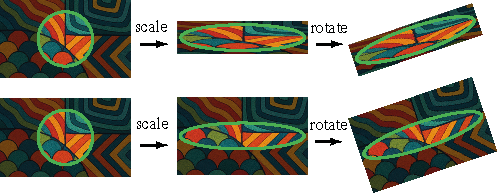
\includegraphics[width=\linewidth]{images/stretch.pdf}
\caption{
\label{fig:stretch}
Difference between two mappings for a primitive having learned a particular texture.
Top row: a naive approach distorts the appearance after the primitive undergoes scaling. Bottom row: in our approach, as texel size is fixed in world space, scaling the primitive only reveals more part of the underlying texture, preserving existing content.
}
\end{figure}
Recall that primitives change size and shape during the optimization process. 
%\Fredo{Avoid long sentences with ";"} 
As a result, with such a texture mapping, the appearance parameters of the texture are coupled with the parameters that control the shape of the primitive. 
During optimization, small changes in the scale of the Gaussians result in changes of all the values of the texture. This can induce local minima in the optimization process that are visible as texture stretching, see Fig.~\ref{fig:stretch} (top).
%to keep appearance the same under small changes in the scale of the Gaussian the optimizer needs to change all the values of the texture. This mapping introduces challenging local minimas in the optimization that manifest as \emph{texture stretching during the optimization.} \TODO{Ideally we would want a toy experiment here to help us with the motivation.}

%\PP{This inherently means that the scale of details that can be represented is tightly tied to the size of the primitives.
%As a primitives grows larger it can represent coarser and coarser details}.
%\PP{To counteract this behavior,
%the only solution is to either dynamically adapt the texture resolution
%or/and add more primitives.}



%as optimization evolves,
%there is a need to balance between adapting texture resolution and adding more primitives.
%Some previous \PP{concurrent, others?} methods use fixed texture resolution ~\cite{bbsplat,textured3dgs};
%\PP{as a result, the only option, the}
%texture resolution/primitive balance is heuristically treated by splitting primitives,
%which results in texture resolution being ``spread out'' across the scene \PP{not sure about this one}.
%Alternatively texture resolution can be adaptively modified based simply on stretching \cite{gstex}.
%These solutions do not take the \emph{content} of the scene in to account, which can result in texture residual stretching and suboptimal distribution of texture resolution.
%\PP{parameter/memory emphasis}
%We illustrate this effect in Fig.~\ref{fig:stretch}(a)-(b).
%\GK{This whole paragraph puzzled me quite a lot: 1) I think "texture resolution" is used very relaxed here, afaik no other related work changes the actual resolution of the texture resolution of the primitives, one can think of adding more primitives increases the "total texture resolution" availiable to the representation but I think the terms are conflated here. 2) I think its dangerous to go through other papers in details in our method because probably reviewers and other readers will not know by heart the literature, and since we have never introduced each other paper in detail it makes the method very hard to read. I would propose to ignore concurrent work until the result section.}
%\TODO{Contrast paragraph with concurrent work, all use (2) we use (3)}
Instead, we define a \emph{content-aware} representation in which textures are adapted to scene content. 
%\Fredo{And discuss positive impact on optimization.}
Our goal is to have textures that can faithfully represent the frequency of image details at the highest resolution present in the input images.
To do this, we fix the texel size with respect to the optimization process such that no optimizable parameters change it. We achieve this with a small modification to Eq.~\ref{eq:basic-u}:
\begin{equation}
    \mvec{u} = \frac{\mvec{p}^l}{k_i} + T_\text{offset}
\end{equation}
\noindent
where $k_i$ is the texel size and $T_\text{offset}$ is an offset to center the texture map.
\revision{rev9584 what does world units mean}{
In constrast to Eq.~\ref{eq:basic-u},
the intersection point $\mvec{p}^l$ and hence the texel size $k_i$ are defined in world space,
with the same units as the primitive's scales $\mvec{\sigma}$.
}

\revision{rev2866 texture resolution unclear}{This mapping implies that the textures do not have a fixed texture resolution.
On the contrary,
as the primitives grow or shrink,
more or less texture resolution is needed to cover their surface.
This is demonstrated in Fig.~\ref{fig:stretch} (bottom).
}
We modified our optimization routines to allocate and de-allocate texture resolution dynamically. %%optimization.

%Changing the scale of a primitive has the sole effect of exposing more or less of same sized texels,
%instead of stretching or contracting them.

Since the number of texels can grow quadratically, we risk running out of resources if every primitive  has a texture. Our goal is to maintain an expressive representation while carefully managing resources. To achieve this, we enforce two properties on our representation: First, the projected sampling frequency of the texture needs to be bounded by the image sampling frequency of the closest camera. This means that the projected texel size should never be smaller than the smallest input pixel that can see it. Second, texel sizes should adapt to \emph{scene content}, i.e., smaller texel sizes should be allocated for high frequency image content.

The first goal can be achieved using a conservative choice to determine minimum texel size as the pixel size back-projected in world space from the input training view closest to the primitive's center $k^p_{\mathrm{min}}$, similarly to \cite{reduced3dgs}.

% \begin{equation}
% \label{eq:kmin}
% {k}^p_{\mathrm{min}} = {w}^p_{\mathrm{min}},
% \end{equation}
% where ${w}^p_{\mathrm{min}}$ is \TODO{PP: complete},
% similarly to the method presented in~\cite{reduced3dgs}. \TODO{PP: say what we do exactly: In practice, we set this value to be 2 times the size of the pixel, which helps avoid aliasing.}

%\PP{I think we should revert to what I've written initially.
%\begin{itemize}
%    \item Introduce the new need of choosing a texel size
%    \item Present our first, 100\% conservative choice
%\end{itemize}
%Our representation/parametrization dictates the selection of a texel size for our primitives.
% Choosing the same texel size for every primitive can pose a problem;
% too big and it can lead to blurry appearance for high-frequency parts of the scene,
% too small and it can cause aliasing for distant views and can be prohibitively memory-intensive.
% So,
% we proceed with the conservative choice,
% which is to use as texel size the pixel size,
% back-projected in world space from the training camera closest to the primitive's center,
% $k = {w}^p_{\mathrm{min}}$,
% similarly to \cite{reduced3dgs}.}

% \PP{
% The choice above ensures that we do not miss any visual detail existing in our training images.
% However,
% the are very few cases
% where the content of the scene is that high frequency
% that a 1-1 correspondance between texels and pixels is needed.
% In contrary,
% in most cases,
% our primitives need to match low frequency content,
% that can be faithfully represented with fewer color samples.
% To allow our primitives to adapt their texture to the frequency content of the input images,
% we extent our texel size by a texel-to-pixel ratio ($t_2p_r$).
% \begin{equation}
%     k = {w}^p_{\mathrm{min}} \cdot \mathrm{t_{2}p}_r
% \end{equation}
% In \cite{gstex, textured3dgs} the texel size is determined at the texture initialisation step,
% and the primitives get assigned a fraction of a total texel budget based on area.
% However,
% this does not take into consideration th
%}

%\PP{we need to discuss this}

%Knowing a-priori the ideal $k_i$ that controls the texel size for each primitive is impractical since primitive scales and distributions dynamically adjust during the optimization. 
Regarding the second goal,
 optimal texel sizes cannot  be determined at initialization
since pritimives change size and rotate dynamically during optimization.
We need a way to adapt to the freqency content of the scene progressively. 
%To that end we introduce during the optimization an adaptive strategy to determine the texel size per primitive. Our method allows to downscale and upscale textures such that regions with high frequency content get allocated textures with smaller texel sizes and low frequency regions coarser textures with larger texel sizes. We build on this observation to propose resolution-aware primitive management.
To do this, we next introduce an adaptive strategy to determine texel size during optimization, where we downscale and upscale texture by adapting to the scene \emph{content}. 
We complement this approach with a resolution-aware primitive management method that add primitives to represent geometric -- rather than appearance -- error.
We describe these two components in the following sections.

%\Fredo{The use of commas "," is often questionable. I have tried to fix it, but be on the lookout. For example, there is usually no comma before that (in contrast to which).}

%We describe the necessary components in the following sections.

% \TODO{I have done until here, took me longer than expected.}
% We could envisage initializing primitive textures by matching resolution from the closest input image. However, we follow standard Gaussian Splatting practice and we initialise our method using the sparse SfM point cloud,  generated during camera calibration. As a result, it would be impractical to initialize all textures using this criterion, since the initial distribution of points (large, non-uniform points etc.) does not provide a sufficient representation of scene geometry. In particular, large points could require very high resolution textures which could be wasteful. 

% Given the need to adapt to frequency content and to progressively achieve resolution matching, 
% we introduce an adaptive strategy to determine texel size during optimization, by introducing a method that allows downscale and upscale of texture. 
% This process provides a set primitives with textures; in regions with large primitives corresponding to high frequency content, required texture resolution will increase. We build on this observation to propose resolution-aware primitive management.
% We describe these two components in the following sections.

% \GK{I think in the last 2-3 paragraphs we are missing an imporant point: We want the texture resolution to be bounded by the matching resolution of the closest image and not necessarily match it since that would be wasteful in cases where the image frequencies are low. }


%%% ADAPT
%In contrary to the above, we chose to define our texture grid on the axis-aligned space, that is, the local coordinates space, in which the axes are scaled by the scales of the primitive, instead of being normalised.  With this formulation the texels have a constant world-space size, independent on the primitive's scale.
%Hence, scaling up or down a primitive has the sole effect of exposing more or less of same sized texels, instead of stretching or contracting a fixed number of them.
%
%This formulation has the advantage of better disentangling the geometry of the primitive, that has to do with its rotation and how big or small it is, from its appearance, as a primitive can grow or shrink without affecting the parts of the scene that it has already fit.
%
%The particularity in this case is that we cannot set the texture resolution, as it changes dynamically with the size of the primitive.  Instead, we need to set the texel size for each primitive.  To avoid choosing a fixed size for all primitives, something that could prove to be too wasteful and aliasing inducing or too coarse and inappropriate,
%depending on the how small or big it would be, we decided to be conservative and choose as texel size the world size width of a pixel, back projected to the centers of our primitives, taken by the closest training camera.  That ensures that on one hand, primitives have the capacity to reconstruct the finest observable details and on the other hand, primitives that are consistently observed from afar do not have too small texels, causing aliasing and wasting memory.
%
%\TODO{that's tricky to explain because it's a bit of an implementation issue. the UV coordinates need some texture resolution to be constrained in the 0-1 range and I think that'll more confusing than just saying, we query our texture like that} The mapping in this case goes directly to the texture indices,
%



%\begin{itemize}
%\item Instead we define a content-aware texture representation in which world-space texel size is adapted to represent the content in the input images.
%\item Diagram showing cases
%\item In practice, texel size needs to be adapted during optimization. We next explain the steps of our method.
%\end{itemize}

\subsection{Progressive Adaptive Texel Size Determination}

%\begin{itemize}
%\item Then we need to do this adaptively Notion of texture detail, requirement of frequency
%\item Have an additional parameter that allows finer control $t2p_r$, adapt to frequency
%\item Then downscale upscale definition
%\item Progressive algorithm: start with 2DGS (500 iterations), warm up wo textures. Then init everyone to 8x8 and compute $t2p_r$, for the next few hundreds of iterations, downscale and upscale will find resolution that is adapted to content.
%\item We next talk about splitting
%\end{itemize}

%The choice of texel size made above is, as already mentioned, conservative to the finest observable detail.
%However, in most cases, primitives do not need that high of a granularity, as they might be in parts of the scene with coarse details.
%In these cases, having approximately one texel per pixel is too wasteful in terms of memory and may also cause optimisation issues due to overparametrisation.

Our goal is to adapt textures to the frequency content of the input images. We also need to achieve this in a progressive manner that fits well with the optimization process. We define a \emph{texel size-to-pixel} size ratio ${t_{2}p}_r$, which we manipulate during optimization using downscaling and upscaling operations.

We define the texel size $k$ based on the minimum pixel size ${k}^p_{\mathrm{min}}$, with ${t_{2}p}_r$ as follows:
\begin{equation}
    k = {k}^p_{\mathrm{min}} \cdot {t_{2}p}_r
\end{equation}

\noindent
%This reparametrisation offers us a knob 
%that we can use to adjust the size of the texels of individual primitives,
%depending on the underlying content of the scene. \TODO{giving us more control on parameter/memory budget}.
We use this parameter to assign a low $t_2p_r$ to primitives in regions with fine details.
% \GK{I don't understand that, let's say you have 1:1 texel to pixel ratio, this means you have one texel to pixel that bounds the frequency of the images, an even lower texel to pixel ratio i.e 1:10 mean you have one texel for 10 pixels - are we sure low here is what we want?}
As a result, such primitives will have more texels for a given primitive size.
Similarly, primitives that lie in areas with low-frequency appearance will have a higher ratio,
giving them relatively fewer texels.
% \GK{do we bound texel-to-pixel ratio  between (0,1]? if we do this is the section to mention it.}
To provide a lower bound of 1 and facilitate texture rescaling operations,
$t_2p_r$ can only take values that are powers of two.

To this end, we propose two strategies to increase and decrease $t_2p_r$
leading to a downscale and an upscale of the texture map respectively.
Note that texel size and texture resolution are linked, but not the same. In the operations below, when texel size changes, texture resolution will change but only because the \emph{primitive size is unchanged}.

\begin{figure}[!h]
	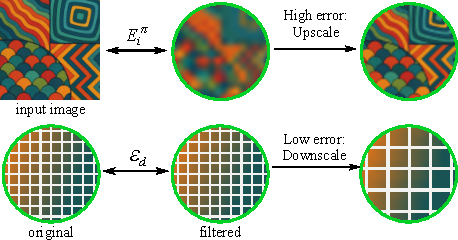
\includegraphics[width=\linewidth]{images/upscale_downscale/updownscale.pdf}
\caption{
\label{fig:down-up}
We illustrate the downscale and upscale process used.
}
\end{figure}

\textbf{Increase of texel size-to-pixel size ratio - Downscaling}:
Our goal is to find texture maps that represent low frequency details and decrease their texel size accordingly.
We do this by applying a low-pass filter on textures and then comparing them to the originals.
The error $\mathcal{E}_d$ is weighted by the Gaussian falloff of the primitive,
leading to the following equation:
\begin{equation}
    \mathcal{E}_d = \frac{1}{\sum_\mvec{p}G(\mvec{p})}\sum_\mvec{p}G(\mvec{p})(T_\mathrm{orig}(\mvec{p}) - T_\mathrm{lowpass}(\mvec{p}))
\end{equation}

If this error is less than a threshold $\tau_\text{ds}$,
we assume that the texture map can be reconstructed with good-enough fidelity by the downscaled version.
Hence, we double  ${t_{2}p}_r$, which
reduces the total number of texture parameters by 4.
This reduces the resolution of texture, since the world-space size of the texels has grown. The size of the primitive is however unchanged. 

\textbf{Decrease of texel size-to-pixel size ratio - Upscaling}:
In regions where the texel size of the primitives involved is too large to capture the fine, underlying details, we expect our images to be blurry, and thus induce large error.
To identify these regions, we estimate primitive error using the approach presented in~\cite{revising}.
Specifically, for a primitive $i$, a ray $\mvec{r}$, a camera view $\pi$ and corresponding RGB error image $\mathcal{E}_\pi$,
we compute the per primitive error for a single view:
\begin{equation}
    E^\pi_i = \sum_{\mvec{r} \in \mathcal{P}_i} \mathcal{E}_\pi(\mvec{r})w^\pi_i(\mvec{r})
\end{equation}
where $\mathcal{P}_i$ are all the pixels covered by the primitive.
%TODO{In a slight abuse of notation,
Here we assume that we have one ray per pixel,
emanating from its center.
Differently from \cite{revising},
instead of taking the maximum error over views, %aggregating the errors across images with a max operator,
we perform a weighted sum,
with the weight being the total contribution of a primitive in that image.
\begin{equation}
    E_i = \frac{\sum_{\mvec{\pi} \in \Pi} E^\pi_i \overline{w_i^\pi}}{\sum_{\mvec{\pi} \in \Pi} \overline{w_i^\pi}}, \quad
    \overline{w_i^\pi} = \sum_{\mvec{r} \in \mathcal{P}_i}w_i^\pi(\mvec{r})
\end{equation}

\noindent
where $\Pi$ is the set of all input views.
%Concisely,
This choice assigns an error value to each primitive that is proportional to their contribution to the rendered image.

We choose the top 10\% of primitives with the highest error, and upscale their textures by a factor of 4,
by halving $t_2p_r$.
With smaller sized texels,
these primitives can better fit to the scene content,
reducing their error.

\textbf{Progressive texel size adaptation.}
The calculation of the per primitive error $E_i$ and
the application of upscale/downscale process happens regularly during optimization.
Texel size adapts to scene content during this process, getting bigger for primitives that lie in low-frequency regions, and smaller for primitives that exhibit large error,
as shown in Fig.~\ref{fig:teaser}(right).
%Specifically for the latter case,
%it is expected that the error associated with a primitive drops as it gets upscaled,
%as more and finer texels are assigned to it and thus it can better fit the content.
%However,
%this is not always the case,
%because the error can appear in regions that are badly reconstructed,
%in terms of geometry i.e. missing objects.

There are two main sources of error: appearance and geometry. For the first case, our upscaling approach reduces error as the optimization progresses.
However, for the case of geometry that is not well represented, an additional step is required.
% To initialize the process,
% we run 500 iterations of 2DGS where each primitive has a single constant color.
% At this point,
% we assign an 8x8 texture to all primitives \PP{we set the $t_2p_r$ of our primitives so that their smallest dimension has 8 texels}, then continue optimization,
% calculating the error and applying the upscale/downscale process every 250 iterations.
% Consequently,
% after a few of these steps,
% some primitives will have high-resolution textures,
% corresponding to regions with fine detail.
% In such cases,
% such primitives often need to be split,
% either to better capture \emph{geometry detail} or to strike a better balance between memory used for primitive parameters and texture offsets.
To address this and complete our content-aware method, we next introduce resolution-aware splitting.

% \begin{itemize}
%     \item The ratio 1 pixel per texel is too wasteful on memory. So let's have multiples of the base
%     \item So we need a way to change the size of texels. We parametrize the texel size as minimum\_pixel\_width * pixel\_texel ratio, where that latter is a power of 2
%     \item Choosing a global texel size is challenging, since 1) not every area has the same scale of details and being conservative is wasteful
%     \item We develop 2 strategies to change this value.
%     \item Increase the texel size (downscale): Downscale our textures by a factor of 2 using bicubic interpolation. Upscale using bicubic interpolation. Compare the reconstructed and the original with an L1 loss * the opacity and the falloff (alpha value). If that loss is small, lower than a threshold, then we assume that the texture is simple enough so the downscaled version can be used. This reduces the memory for a particular texture by a factor of 4!
%     \item Decrease the texel size (upscale): As this has an effect on memory, we want to do it only in regions where it's needed. And what's a better criterion than the actual error we optimise for??? So we compute this error from all views, weighted by the primitives' contributions. We then pick the 10\% of primitives with the highest error and we upscale them by a factor of 2, using nearest neighbour interpolation, to have zero-effect on the scene. This increases the memory of a particular texture by a factor of 4.
%     We set set the minimum pixel\_texel\_ratio to 2, because we noticed that blending allows to get details of subtexel scale, by combining colours from multiple primitives, so we don't lose any expressivity.
% \end{itemize}
    
\subsection{Resolution-aware Primitive Management}
% \PP{Need to discuss this
% I like the 3 paragraphs.
% However, I prefer the layout I had made,
% 1)"Adaptive texel size to match appearance" (previous section)
% 2)"Densification to add points" (the standard SfM is too sparse and not even our super points can deal with that sparseness + flat planes approximation; no one will tell us off because we didn't give a better intuition on why we need densification, not even original 3dgs explained in-depth why.)
% 3)Since our error is RGB, we use texture resolution as threshold (these 3 paragraphs),
% implying that if we had both RGB and geometric error this wouldn't be necessary (never tested, unfortunately, but is very probably true).
% On the other hand I can get that this might be too complicated.
% }

%Even with our more expressive points,
%this point cloud is too sparse,
%so we also need to employ Adaptive Density Control (ADC)
%to add points in parts of the scene that are not well reconstructed.
%Because our primitives are more expressive and carry more parameters with them,
%cloning strategies used by the original method and others
%\cite{Kerbl_2023}
%\missingcitation{MCMC, 3dgs, revising},
%that work by stacking points on top of each other
%are not appropriate.
%Instead,
%we opted for a splitting strategy, similar to the \missingcitation{revising densification} one.
%
%In the same way as in the upscaling strategy,
%for the 10\% primitives with the highest error
%we check which of those exceed a size threshold.
%These primitives get replaced by two primitives,
%displaced by +- 1 size (std),
%having half the respective scale
%and $G(1)$ the opacity.
%
%The texture grids of the newly added points results from the original one by sampling it at the respective locations.
%
% \begin{itemize}
%     \item The initial point cloud is too sparse. We need a way to add points.
%     \item The original cloning method or other methods that are based on cloning like MCMC \missingcitation{mcmc} have the undesireable effect of stacking a lot of points on top of each other. As our primitives are heavier in terms of parameters and in general, can overfit more easily, such a strategy proved to be unsuitable, both in terms of memory and quality
%     \item However, with our new primitives we can construct a better splitting strategy. Let's define the properties that we want to have.
%     1) Primitives that well reconstruct their part of the scene should remain untouched
%     2) Primitives that reconstruct their part of the scene badly should be spilt into smaller primitives that add more degrees of freedom in terms of geometry, and hence are more flexible.
%     3) To avoid adding too many primitives and flocking the optimiser with parameters, we want to apply that to primitives that have a size greater than a threshold
%     \item So primitives above a size and error threshold get split into two, along the overflowing dimension.
% \end{itemize}

%The choice of this size threshold is discussed in the next section.

%\subsection{Source of errors and Interplay}

% During optimisation, we don't know why a primitive has error.
% There are 2 cases.
% 1) the primitive has the correct appearance, but doesn't match the geometry. Since we have flat primitives, that means that they might protrude/poke out from some views. In this case we need more fine-grained geometry, which can be achieved by getting more points
% 2) the primitive matches the surface but doesn't match the appearance. This case didn't exist in the original method since the number of colour and geometric samples was tied. In our case, though, we can deal that by increasing the colour samples, something that can be done by reducing the texel\_pixel\_ratio
%\TODO{maybe put it in the beginning, as a discussion, in a more "general" way. Like, let's say we have primitives that can match the appearance and geometry separately, describe what we want, and then proceed into the two methods that actually do this}



In Gaussian splatting methods where each primitive contains one color sample, \emph{densification} -- i.e., adding new primitives through cloning and splitting -- plays an essential role in improving the reconstruction of the scene.
This results in a local increase in both the geometric (position, scale, rotation) and appearance parameters (SH, opacity) that are treated together since they are tied to a single Gaussian primitive. 
%hence increasing, locally,
%both the geometric and the appearance degrees of freedom/parameters.
However, this is not always ideal, since there are cases where the geometry is low frequency and has been approximated well, but we are missing texture detail, or conversely, cases where the color information is low frequency, but the underlying surface is not correctly represented. The latter case can appears as holes, ``softened'' edges or elongated primitives in places where they are not required. 

\begin{figure}[!h]

\includegraphics[width=\linewidth]{images/split.pdf} 
\caption{
\label{fig:splitting}
Left to right:The primitive has been upscaled to a resolution greater than $\tau_{tr}$ in both axes. Our splitting approach creates four new primitives, each with half the scale and texture resolution in both axes.}
\end{figure}


Our separation of geometric and appearance parameters provides an additional degree of freedom, allowing us to independently decide whether to increase the number of parameters linked to \emph{geometry}, i.e., increasing the number of primitives or to \emph{appearance}, i.e., increasing texture resolution.

Given that we do not have a supervision signal explicitly for geometry, 
%In our framework,
%we can use the two strategies introduced in sections and 
%to essentially inject geometric and appearance parameters \textbf{separately} to our scenes,
%to address these two sources of error.
%For the first one we can upscale the respective primitives to add more colour samples,
%while for the second one,
%we can split the existing primitives to add more geometric degrees of freedom.
%However,
%since our representation is supervised by the appearance (we don't use any geometric supervision),
we attempt to first match the appearance, using the upscaling approach described above.
If the error is still high despite upscaling,
we interpret the remaining error as geometric.
In these cases,
we can add more primitives,
locally increasing the geometric degrees of freedom.
\revision{rev2866 3dgs-mcmc}{
We found that densification strategies that were based on cloning either partially \cite{3dgs} or entirely in the case of 3DGS-MCMC \cite{3dgs-mcmc}, are incompatible with our representation. This is because
the superimposition of multiple textured primitives makes convergence difficult and requires an excessive number of parameters.
As a result our primitive management is based on \emph{splitting}, which fits well with our method. We describe this next.
%that is adjusted to the rest of the framework and is described next.
}

%And that is done by taking the texture resolution as the size threshold.

Similar to the approach for upscaling, we take the top 10\% of primitives with the highest error, and check which of these exceed a threshold $\tau_{\mathrm{tr}}$ for texture resolution. The primitive is replaced by two new primitives, each displaced by $\pm 1$ standard deviation of the Gaussian.
This process is performed separately for each axis; the new primitives have half the scale (size) in each corresponding axis,
as a result, half the texture resolution,
$G(1)$ times the opacity, where $G$ is the Gaussian.
The texture map of the newly added primitives is created by sampling the original point at the respective locations.
Fig.~\ref{fig:splitting} illustrates the splitting process for a primitive that happens to have a texture resolution greater than $\tau_{\mathrm{tr}}$ in both axes. A flowchart of how upscaling and splitting interact is shown in Fig.~\ref{fig:densify}. Alg.~\ref{alg:routines} displays in high level how the two methods are integrated in code.

\begin{figure}[!h]
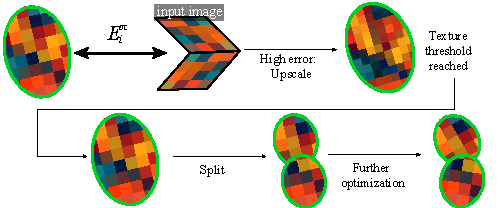
\includegraphics[width=\linewidth]{images/densify/densify.pdf} 
\caption{
\label{fig:densify}
The primitive has high error, and successive upscalings result in a texture resolution above threshold. In this case, the error is geometric rather than due to appearance. Our algorithm performs a split, and further optimization will match the geometry.}
\end{figure}


% With the upscaling strategy described above,
% our primitives can acquire complex appearances to match the underlying scene content.
% For that to happen though,
% it is imperative that the primitives approximate the underlying geometry well,
% because otherwise multi-view inconsistencies can hinder or even entirely prevent the learning of one, consistent appearance.
% As our primitives are flat,
% they can only provide a planar approximation of the surfaces,
% the granularity \TODO{find a better word?} of which depends on the primitives' sizes.
% However,
% in cases where the primitive density is low,
% either due to the initialisation or the optimisation procedure,
% and does not allow the primitives to become small (as there would be holes otherwise),
% we need a way to add new points,
% that is compatible to our representation.
% More specifically,
% since our primitives are more expressive and carry more parameters with them,
% cloning strategies used by the original method and others \missingcitation{MCMC, 3dgs, revising},
% that work by stacking points on top of each other
% are note appropriate.


% Since this complicates both strategies of adaptive texel size and adding new points,
% we decided to create a link between the two,
% to create an interplay.
% This link is choosing the size of the splitting criterion to be the texture resolution of a primitive.

% In that way,
% a primitive without error is left unaltered.
% If a primitive has error,
% this strategy will first try to correct that by assigning more colour samples to it, increasing its resolution.
% If this gets too high, then the primitive will be split into multiple primitives,
% each one having a fraction of the original resolution.
% These smaller primitives can attach themselves better to surfaces,
% and since they represent more localised appearance,
% they can have simpler textures,
% enabling downscaling.


\begin{table*}[!ht]
\footnotesize
\setlength\tabcolsep{1.5pt}
\centering
\scalebox{0.85}{
\begin{tabular}{@{}>{\raggedright\arraybackslash}p{1.8cm}|>{\centering\arraybackslash}p{0.8cm}>{\centering\arraybackslash}p{0.8cm}>{\centering\arraybackslash}p{0.8cm}>{\centering\arraybackslash}p{0.8cm}>{\raggedleft\arraybackslash}p{0.8cm}>{\centering\arraybackslash}p{0.9cm}>{\centering\arraybackslash}p{0.55cm}|>{\centering\arraybackslash}p{0.8cm}>{\centering\arraybackslash}p{0.8cm}>{\centering\arraybackslash}p{0.8cm}>{\centering\arraybackslash}p{0.8cm}>{\raggedleft\arraybackslash}p{0.8cm}>{\centering\arraybackslash}p{0.9cm}>{\centering\arraybackslash}p{0.55cm}|>{\centering\arraybackslash}p{0.8cm}>{\centering\arraybackslash}p{0.8cm}>{\centering\arraybackslash}p{0.8cm}>{\centering\arraybackslash}p{0.8cm}>{\raggedleft\arraybackslash}p{0.8cm}>{\centering\arraybackslash}p{0.9cm}>{\centering\arraybackslash}p{0.55cm}}
 & \multicolumn{7}{c|}{DeepBlending} & \multicolumn{7}{c|}{Mip-Nerf-360} & \multicolumn{7}{c}{Tanks\&Temples} \\
 & SSIM$\uparrow$ & PSNR$\uparrow$ & LPIPS$\downarrow$ & Points & Texels & Params & FPS & SSIM$\uparrow$ & PSNR$\uparrow$ & LPIPS$\downarrow$ & Points & Texels & Params & FPS & SSIM$\uparrow$ & PSNR$\uparrow$ & LPIPS$\downarrow$ & Points & Texels & Params & FPS \\
\midrule
3DGS-MCMC &  0.903 & 29.81 & 0.311 & 1323K & 0.0M & 78.1M & 265 & 0.831 & 27.82 & 0.232 & 2587K & 0.0M & 152.6M & 103 & 0.855 & 24.25 & 0.211 & 695K & 0.0M & 41.1M & 230 \\
\midrule
2DGS* & {\cellcolor{tabthird}} 0.899 & {\cellcolor{tabthird}} 29.52 & 0.324 & 1444K & 0.0M & {\cellcolor{tabsecond}} 83.8M & {\cellcolor{tabfirst}} 96 & {\cellcolor{tabsecond}} 0.801 & {\cellcolor{tabfirst}} 27.18 & {\cellcolor{tabthird}} 0.282 & 2079K & 0.0M & {\cellcolor{tabfirst}} 120.6M & {\cellcolor{tabfirst}} 91 & 0.834 & 23.37 & {\cellcolor{tabthird}} 0.239 & 872K & 0.0M & {\cellcolor{tabsecond}} 50.6M & {\cellcolor{tabfirst}} 165 \\
BBSplat & 0.898 & 29.25 & {\cellcolor{tabsecond}} 0.318 & 160K & 41.0M & 173.0M & {\cellcolor{tabthird}} 27 & 0.781 & 26.67 & {\cellcolor{tabsecond}} 0.273 & 237K & 60.9M & 257.0M & {\cellcolor{tabthird}} 23 & {\cellcolor{tabfirst}} 0.848 & {\cellcolor{tabfirst}} 23.62 & {\cellcolor{tabfirst}} 0.178 & 300K & 76.8M & 324.3M & {\cellcolor{tabthird}} 38 \\
GSTex & {\cellcolor{tabsecond}} 0.906 & {\cellcolor{tabsecond}} 29.63 & {\cellcolor{tabthird}} 0.323 & 1503K & 10.0M & {\cellcolor{tabthird}} 117.2M & 21 & {\cellcolor{tabfirst}} 0.802 & {\cellcolor{tabsecond}} 27.06 & 0.285 & 2025K & 10.0M & {\cellcolor{tabsecond}} 147.5M & 20 & {\cellcolor{tabsecond}} 0.842 & {\cellcolor{tabsecond}} 23.48 & 0.240 & 877K & 10.0M & {\cellcolor{tabthird}} 80.9M & 20 \\
Ours & {\cellcolor{tabfirst}} 0.907 & {\cellcolor{tabfirst}} 30.03 & {\cellcolor{tabfirst}} 0.303 & 222K & 21.6M & {\cellcolor{tabfirst}} 78.1M & {\cellcolor{tabsecond}} 70 & {\cellcolor{tabthird}} 0.795 & {\cellcolor{tabthird}} 27.00 & {\cellcolor{tabfirst}} 0.263 & 218K & 46.6M & {\cellcolor{tabthird}} 152.6M & {\cellcolor{tabsecond}} 67 & {\cellcolor{tabthird}} 0.835 & {\cellcolor{tabthird}} 23.43 & {\cellcolor{tabsecond}} 0.225 & 164K & 10.4M & {\cellcolor{tabfirst}} 41.1M & {\cellcolor{tabsecond}} 121 \\
\end{tabular}
}

\caption{\label{tab:default-eval}
We compare our method against 2DGS* trained with no geometric regularisations,
BBSplat and GSTex, with default settings.
We show standard quality metrics (PSNR, SSIM, L-PIPS), total number of primitives, texels and parameters.
Our method achieves competitive results while using significantly fewer, highly expressive primitives. \revision{}{We also include 3DGS-MCMC for completeness; please note that 3DGS-based methods achieve better NVS but worse geometry quality compared to all approaches based on 2DGS (see discussion Sec.~\ref{sec:eval}).} }

\end{table*}

\begin{table*}[!ht]
\footnotesize
\setlength\tabcolsep{2pt}
\centering
\scalebox{0.85}{
\begin{tabular}{@{}>{\raggedright\arraybackslash}p{1.1cm}|>{\centering\arraybackslash}p{0.8cm}>{\centering\arraybackslash}p{0.8cm}>{\centering\arraybackslash}p{0.8cm}>{\centering\arraybackslash}p{0.8cm}>{\raggedleft\arraybackslash}p{0.8cm}>{\centering\arraybackslash}p{0.9cm}>{\centering\arraybackslash}p{0.55cm}|>{\centering\arraybackslash}p{0.8cm}>{\centering\arraybackslash}p{0.8cm}>{\centering\arraybackslash}p{0.8cm}>{\centering\arraybackslash}p{0.8cm}>{\raggedleft\arraybackslash}p{0.8cm}>{\centering\arraybackslash}p{0.9cm}>{\centering\arraybackslash}p{0.55cm}|>{\centering\arraybackslash}p{0.8cm}>{\centering\arraybackslash}p{0.8cm}>{\centering\arraybackslash}p{0.8cm}>{\centering\arraybackslash}p{0.8cm}>{\raggedleft\arraybackslash}p{0.8cm}>{\centering\arraybackslash}p{0.9cm}>{\centering\arraybackslash}p{0.55cm}}
 & \multicolumn{7}{c|}{DeepBlending} & \multicolumn{7}{c|}{Mip-Nerf-360} & \multicolumn{7}{c}{Tanks\&Temples} \\
 & SSIM$\uparrow$ & PSNR$\uparrow$ & LPIPS$\downarrow$ & Points & Texels & Params & FPS & SSIM$\uparrow$ & PSNR$\uparrow$ & LPIPS$\downarrow$ & Points & Texels & Params & FPS & SSIM$\uparrow$ & PSNR$\uparrow$ & LPIPS$\downarrow$ & Points & Texels & Params & FPS \\
\midrule
BBSplat & {\cellcolor{tabthird}} 0.895 & {\cellcolor{tabsecond}} 28.93 & {\cellcolor{tabsecond}} 0.332 & 72K & 18.5M & 78.1M & {\cellcolor{tabthird}} 57 & {\cellcolor{tabsecond}} 0.768 & {\cellcolor{tabsecond}} 26.02 & {\cellcolor{tabsecond}} 0.291 & 141K & 36.1M & 152.6M & {\cellcolor{tabthird}} 33 & {\cellcolor{tabsecond}} 0.801 & {\cellcolor{tabsecond}} 22.77 & {\cellcolor{tabsecond}} 0.259 & 47K & 12.3M & 51.8M & {\cellcolor{tabsecond}} 87 \\
GSTex & {\cellcolor{tabsecond}} 0.896 & {\cellcolor{tabthird}} 28.29 & {\cellcolor{tabthird}} 0.354 & 222K & 21.6M & 78.1M & {\cellcolor{tabsecond}} 60 & {\cellcolor{tabthird}} 0.748 & {\cellcolor{tabthird}} 25.19 & {\cellcolor{tabthird}} 0.352 & 217K & 46.6M & 152.6M & {\cellcolor{tabsecond}} 46 & {\cellcolor{tabthird}} 0.745 & {\cellcolor{tabthird}} 20.65 & {\cellcolor{tabthird}} 0.363 & 164K & 10.4M & 41.1M & {\cellcolor{tabthird}} 67 \\
Ours & {\cellcolor{tabfirst}} 0.907 & {\cellcolor{tabfirst}} 30.03 & {\cellcolor{tabfirst}} 0.303 & 222K & 21.6M & 78.1M & {\cellcolor{tabfirst}} 70 & {\cellcolor{tabfirst}} 0.795 & {\cellcolor{tabfirst}} 27.00 & {\cellcolor{tabfirst}} 0.263 & 218K & 46.6M & 152.6M & {\cellcolor{tabfirst}} 67 & {\cellcolor{tabfirst}} 0.835 & {\cellcolor{tabfirst}} 23.43 & {\cellcolor{tabfirst}} 0.225 & 164K & 10.4M & 41.1M & {\cellcolor{tabfirst}} 121 \\
\end{tabular}
}


\caption{\label{tab:same-param-eval}
We compare against BBSplat and GSTex in a same parameter setting,
by adjusting their primitive count and texels accordingly.
The slight discrepancy in BBSplat's parameters in Tanks \& Temples is due to a sphere sampling method they use to model the background and distant objects.
}
\end{table*}


\subsection{Training and Regularisation}
As in \cite{3dgs},
we train our model using the weighted sum of the per-pixel $\mathcal{L}_1$
and the structural similarity losses,
between the ground truth and the rendered images:
\begin{equation}
    \mathcal{L}_{\text{RGB}} = (1-\lambda_{\text{SSIM}})\mathcal{L}_1 + \lambda_{\text{SSIM}}\mathcal{L}_{\text{SSIM}}
\end{equation}
with $\lambda_{\text{SSIM}}=0.2$.

We observed that textures could finish converging to high-frequency settings,
even though alpha-blending would create a smooth result.
This prevented them from being downscaled,
leading to high parameter usage.
To resolve this,
we apply a sparsity regularization on the texel values,
pushing them towards zero,
\begin{equation}
    \mathcal{L}_{\text{texture}} = \lambda_{\text{texture}} \sum_i |\mvec{c}_i^{\mathcal{T}_i}|
\end{equation}
We constrain the texel values in the $[-1,1]$ range,
using a sigmoid activation,
scaled and shifted accordingly:
\begin{equation}
    \mvec{c}^{\mathcal{T}_i} = 2\sigma(\mvec{c}'^{\mathcal{T}_i})-1
\end{equation}
where $\sigma(x)$ is the sigmoid function and $\mvec{c}'^{\mathcal{T}_i}$ are the unactivated texture features.
Intuitively,
this parametrization coupled with the sparsity loss
forces the view-dependent color $\mvec{SH}(\mvec{d})$ to learn the base color of the surface,
while the texels operate as offsets to model high-frequency details.
An example of this is illustrated in Fig.~\ref{fig:teaser}(left).

Finally,
as in \cite{reduced3dgs, 3dgs-mcmc},
we incentivize low-contribution primitives to effectively disappear by applying an opacity regularization term:
\begin{equation}
    \mathcal{L}_{\text{opacity}} = \lambda_{\text{opacity}} \frac{1}{N}\sum_i^N \mvec{o}_i.
\end{equation}

Taking both training objectives and regularizations into consideration,
the total loss is formed as:
\begin{equation}
    \mathcal{L} = \mathcal{L}_{\text{RGB}} + \mathcal{L}_{\text{texture}} + \mathcal{L}_{\text{opacity}}.
\end{equation}

\begin{figure*}[!h]
\centering
\setlength{\tabcolsep}{1.5pt}

    \newcommand{\resultfigwidth}{.193\textwidth}
	\begin{tabular}{cc|cccc}
		& Ground Truth & 2DGS* & BBSplat & GStex & Ours \\
        \raisebox{0.25\height}{\rotatebox{90}{\small Mip-Nerf360}} &
        \spyimage{red}{\resultfigwidth}{images/table1/m360_gt.jpg}{0.4, 1.5}{1.1, 0.6} &
        \spyimage{red}{\resultfigwidth}{images/table1/m360_2dgs_no_regul.jpg}{0.4, 1.5}{1.1, 0.6} &
        \spyimage{red}{\resultfigwidth}{images/table1/m360_bbsplat_baseline.jpg}{0.4, 1.5}{1.1, 0.6} &
        \spyimage{red}{\resultfigwidth}{images/table1/m360_gstex_output_1e7.jpg}{0.4, 1.5}{1.1, 0.6} &
        \spyimage{red}{\resultfigwidth}{images/table1/m360_texture-proj_final_new_downscale_threshold_0.02.jpg}{0.4, 1.5}{1.1, 0.6} \\
		
        \raisebox{0.18\height}{\rotatebox{90}{\small Deep Blending}} &
        \spyimage{red}{\resultfigwidth}{images/table1/db_gt.jpg}{3, 0.3}{3.3, 1.3} &
        \spyimage{red}{\resultfigwidth}{images/table1/db_2dgs_no_regul.jpg}{3, 0.3}{3.3, 1.3} &
        \spyimage{red}{\resultfigwidth}{images/table1/db_bbsplat_baseline.jpg}{3, 0.3}{3.3, 1.3} &
        \spyimage{red}{\resultfigwidth}{images/table1/db_gstex_output_1e7.jpg}{3, 0.3}{3.3, 1.3} &
        \spyimage{red}{\resultfigwidth}{images/table1/db_texture-proj_final_new_downscale_threshold_0.02.jpg}{3, 0.3}{3.3, 1.3} \\

        \rotatebox{90}{\small Tanks\&Temples} &
        \spyimage{red}{\resultfigwidth}{images/table1/tnt_gt.jpg}{3.1, 1.65}{3.1, 0.6} &
        \spyimage{red}{\resultfigwidth}{images/table1/tnt_2dgs_no_regul.jpg}{3.1, 1.65}{3.1, 0.6} &
        \spyimage{red}{\resultfigwidth}{images/table1/tnt_bbsplat_baseline.jpg}{3.1, 1.65}{3.1, 0.6} &
        \spyimage{red}{\resultfigwidth}{images/table1/tnt_gstex_output_1e7.jpg}{3.1, 1.65}{3.1, 0.6} &
        \spyimage{red}{\resultfigwidth}{images/table1/tnt_texture-proj_final_new_downscale_threshold_0.02.jpg}{3.1, 1.65}{3.1, 0.6} \\
	\end{tabular}
\caption{
\label{fig:default-eval}
We provide renderings from one scene per dataset for every method,
trained with default settings.
Our method is able to reconstruct high frequency details on images,
even while using fewer parameters compared to the other methods.
}
\end{figure*}



\section{Implementation}
We have implemented our method using the 3DGS codebase, introducing 2D primitives as in 2DGS. 
%\PP{we used 3dgs and then added bits of 2dgs}.
Unlike 2DGS,
we do not use the $\mathbb{R}^2 \rightarrow \mathbb{R}^2$ transformation to find the intersection point using three non-parallel planes.
Instead, we use Eq.~\ref{eq:intersection_point} directly in camera space.
We did not observe any instability issues.
\revision{rev6315 runtime performance}{
Since our method requires per-ray querying of texture maps,
 both the forward and backward passes incur additional overhead,
that is not compensated by the smaller number of primitives rendered.
In general, compared to 2DGS,
 training time is 1.5-2 times longer, and rendering is 25\% slower.
}

As the texture grids can have different resolutions,
we created custom ``jagged'' tensor data structure to be used for their storage.
The texture resolution for each primitive gets (de-)allocated dynamically,
so that it covers the extent of the primitive,
that is $\pm$3 standard deviations.
This dynamic memory management happens every 100 iterations.
A hard limit of 256 texture resolution is enforced to avoid using too much memory.
When a primitive grows outside of its allocated texture grid,
either because memory has not been allocated yet or it has surpassed the hard limit,
zero-padding is used. Since we are storing an offset, zero-padding reduces to the DC color.

We observed that limiting the $t_2p_r$ to be greater or equal to 2 did not have a detrimental effect on the visual quality,
as subtexel scaled details can be retrieved
thanks to alpha blending and the overlap of our primitives.
%So,
We thus allow upscaling to happen only for primitives with a $t_2p_r$ greater or equal to 2.
% The error calculation,
% adaptive texel size determination and resolution-aware primitive management strategies run every 250 iterations,
% until 25k iterations.
% The threshold $\tau_{\mathrm{tr}}$ starts at $64$ and is progressively reduced to $32$ within 7000 iterations.

% The texture grids are initialized with a value of $0$ on every channel
% and start optimizing after 500 iterations.
% To avoid running out of memory and to avoid early overfitting,
% at 500 iterations,
% we set $t_2p_r$ for each primivite so that their smallest axis is 8 texels wide,
% in practice using the closest power of two value.

% We implement downscaling and upscaling using pytorch's interpolate function,
% with a scale factor of 2,
% which translates to reductions or increases of the number of texels by a factor of 4,
% respectively.
% Upscale is done using nearest neighbour interpolation,
% so that we avoid changing the appearance of the texture,
% that could disrupt that optimizer.



\revision{rev4160 memory/storage}
{
\textbf{Storage and Memory Considerations.}
The size of our representation is tied to the number of parameters used,
with each parameter saved as a 4-byte float,
as in previous Gaussian Splatting implementations.
However,
%as our representation constitutes an extension to the original one,
%we expect 
most Gaussian Splatting compression techniques (see \cite{3dgszip}) are 
applicable to our approach either directly or with minor modifications.
For our newly introduced texture maps,
our choice to use a sigmoid activation to limit the effective range of the texel values allows for a very efficient application of K-means clustering compression. Please see Tab.~\ref{tab:per-scene} for complete statistics.
}

\section{Results and Evaluation}

We test our method on 13 indoor and outdoor scenes from three different standard datasets.
We evaluate on all scenes of Mip-NeRF 360 \cite{mipnerf360},
two scenes from Tanks \& Temples \cite{tnt},
as well as two scenes from Deep Blending \cite{db}.
Fig.~\ref{fig:default-eval} shows that our method faithfully reconstructs the input images.
%\Fredo{Should we discuss how we normalize and keep comparison fair wrt number of primitives vs memory size?}
% \begin{itemize}
% \item Fig. \ref{fig:results} line showing our result and GT on 2 scenes
% \item Show that quality is good
% \item Give Speed, memory etc.
% \end{itemize}

\subsection{Evaluation}
\label{sec:eval}

We compare our method against 2DGS \cite{2dgs} as a baseline,
and two 2DGS texturing methods,
namely (unpublished) BBSplat~\cite{bbsplat} and GStex \cite{gstex},
for which the code was available at the time of submission.
\revision{rev9584 2866 comparison to textured-3dgs 3dgs-mcmc}
{
Directly comparing to 3DGS-based models is not straightforward and might lead to misleading conclusions,
since these models have different properties and consistently perform better for NVS but worse in geometry reconstruction,
compared to 2DGS-based solutions~\cite{2dgs}.
For the same reason,
and because the code was not available at the time of submission,
we do not compare against \cite{textured3dgs},
which is a 3DGS-based method with textured primitives.
This model uses a pretrained 3DGS-MCMC model as initialization,
similar to GStex,
and includes RGBA textures,
similar to BBSplat.
We thus expect it to suffer from the disadvantages of both these two models (see discussion of the second experiment).
}
We ran these methods on all scenes using our machines to ensure fair comparison.
For 2DGS,
the normal consistency and depth distortion regularization terms were disabled,
as they are designed to enhance the geometric reconstruction
but often result in lower novel view synthesis (NVS) quality.

\begin{figure*}[!h]
\centering
\setlength{\tabcolsep}{1.5pt}

    \newcommand{\resultfigwidth}{.24\textwidth}

\begin{tabular}{cc|ccc}
    & Ground Truth & BBSplat & GStex & Ours \\
    \raisebox{0.4\height}{\rotatebox{90}{\small Mip-Nerf360}} &
    \spyimage{red}{\resultfigwidth}{images/table2/m360_gt.jpg}{1.4, 2.5}{1.1, 0.7} &
    \spyimage{red}{\resultfigwidth}{images/table2/m360_bbsplat_same_params_.jpg}{1.4, 2.5}{1.1, 0.7} &
    \spyimage{red}{\resultfigwidth}{images/table2/m360_gstex_output_same_params.jpg}{1.4, 2.5}{1.1, 0.7} &
    \spyimage{red}{\resultfigwidth}{images/table2/m360_texture-proj_final_new_downscale_threshold_0.02.jpg}{1.4, 2.5}{1.1, 0.7} \\
    
    \raisebox{0.3\height}{\rotatebox{90}{\small Deep Blending}} &
    \spyimage{red}{\resultfigwidth}{images/table2/db_gt.jpg}{2.5, 0.3}{4, 0.7} &
    \spyimage{red}{\resultfigwidth}{images/table2/db_bbsplat_same_params_.jpg}{2.5, 0.3}{4, 0.7} &
    \spyimage{red}{\resultfigwidth}{images/table2/db_gstex_output_same_params.jpg}{2.5, 0.3}{4, 0.7} &
    \spyimage{red}{\resultfigwidth}{images/table2/db_texture-proj_final_new_downscale_threshold_0.02.jpg}{2.5, 0.3}{4, 0.7} \\

    \raisebox{0.15\height}{\rotatebox{90}{\small Tanks\&Temples}} &
    \spyimage{red}{\resultfigwidth}{images/table2/tnt_gt.jpg}{2.1, 0.1}{1.1, 0.7} &
    \spyimage{red}{\resultfigwidth}{images/table2/tnt_bbsplat_same_params_.jpg}{2.1, 0.1}{1.1, 0.7} &
    \spyimage{red}{\resultfigwidth}{images/table2/tnt_gstex_output_same_params.jpg}{2.1, 0.1}{1.1, 0.7} &
    \spyimage{red}{\resultfigwidth}{images/table2/tnt_texture-proj_final_new_downscale_threshold_0.02.jpg}{2.1, 0.1}{1.1, 0.7} \\
\end{tabular}

\caption{
\label{fig:same-param-eval}
Adjusting BBSplat and GSTex to use the same budget as our method, results in significant visual degradation.}
\end{figure*}

\textbf{Qualitative Evaluation.}
%\Fredo{Sentence hard to parse. Simplify. Check I didn't break it. Is the end of the sentence useful?} 
In Figure~\ref{fig:default-eval},
we show visual results for the different models. We show
test views (i.e., not used for training) from one scene of each dataset.
Our method succeeds in reconstructing high-frequency details with high fidelity,
even with fewer parameters.
Similarly, Figure~\ref{fig:same-param-eval} displays visual results from the second experiment,
which highlight that other texturing methods struggle when constrained to the same parameter budget as ours.
GSTex uses a point cloud that is not trained with textured primitives in mind
and a static heuristic distribution of texels, which causes it to
not reconstruct well large parts of the scene.
BBSplat succeeds in geometrically reconstructing the scene, but exhibits texture stretching, which appears as blurriness.
This is due to the choice of mapping between intersection points and UV coordinates. 
%\Fredo{Hard to parse, long winded, rephrase}

%\subsection{Evaluation}
\textbf{Quantitative Evaluation.}
For our quantitative comparisons,
we present results for three error metrics, SSIM, PSNR, and LPIPS \cite{lpips},
that are typically used to evaluate NVS.
Additionally,
we report the number of primitives and
texels used,
which provides a precise measure of the resources required for each method
and demonstrates whether and how much textures contribute to the scene reconstruction.
\revision{rev9584 scope of the paper, primitive vs parameters}{
Finally,
since the models' capacity is directly tied to the number of parameters used,
we include the relevant column so that we can make fair comparisons and draw meaningful conclusions.
}

\revision{rev4160}{
The formula for the number of parameters differs slightly among the models.
}
For 2DGS, GSTex each primitive has 58 parameters (3 for position, 2 for scale, 4 for rotation, 1 for opacity, 48 for color),
while for BBSplat this number is 57,
as it lacks opacity.
In our method,
in addition to the parameters of 2DGS,
we include one additional per primitive for the texel size,
pushing the number to 59 parameters.
Regarding the parameters coming from texels,
GSTex and our method have 3 per texel,
while BBSplat has one additional,
corresponding to the alpha channel.


\begin{table*}[!ht]
\footnotesize
\setlength\tabcolsep{2pt}
\centering
\begin{tabular}{@{}>{\raggedright\arraybackslash}p{1.3cm}|>{\centering\arraybackslash}p{0.8cm}>{\centering\arraybackslash}p{0.8cm}>{\centering\arraybackslash}p{0.8cm}>{\raggedleft\arraybackslash}p{0.7cm}>{\centering\arraybackslash}p{0.9cm}>{\centering\arraybackslash}p{0.6cm}|>{\centering\arraybackslash}p{0.8cm}>{\centering\arraybackslash}p{0.8cm}>{\centering\arraybackslash}p{0.8cm}>{\raggedleft\arraybackslash}p{0.7cm}>{\centering\arraybackslash}p{0.9cm}>{\centering\arraybackslash}p{0.6cm}|>{\centering\arraybackslash}p{0.8cm}>{\centering\arraybackslash}p{0.8cm}>{\centering\arraybackslash}p{0.8cm}>{\raggedleft\arraybackslash}p{0.7cm}>{\centering\arraybackslash}p{0.9cm}>{\centering\arraybackslash}p{0.6cm}}
 & \multicolumn{6}{c|}{DeepBlending} & \multicolumn{6}{c|}{Mip-Nerf-360} & \multicolumn{6}{c}{Tanks\&Temples} \\
 & SSIM$\uparrow$ & PSNR$\uparrow$ & LPIPS$\downarrow$ & Texels & Params & FPS & SSIM$\uparrow$ & PSNR$\uparrow$ & LPIPS$\downarrow$ & Texels & Params & FPS & SSIM$\uparrow$ & PSNR$\uparrow$ & LPIPS$\downarrow$ & Texels & Params & FPS \\
\midrule
Points40k & 0.890 & 28.78 & 0.346 & 13.2M & 41.9M & 121 & 0.758 & 25.80 & 0.304 & 42.2M & 128.9M & 97 & 0.809 & 22.74 & 0.246 & 15.4M & 48.4M & 162 \\
Points80k & {\cellcolor{tabthird}} 0.898 & {\cellcolor{tabthird}} 29.56 & {\cellcolor{tabthird}} 0.328 & 15.5M & 51.2M & 88 & {\cellcolor{tabthird}} 0.777 & {\cellcolor{tabthird}} 26.39 & {\cellcolor{tabthird}} 0.285 & 43.9M & 136.5M & 79 & {\cellcolor{tabthird}} 0.823 & {\cellcolor{tabthird}} 23.25 & {\cellcolor{tabthird}} 0.235 & 12.3M & 41.7M & 108 \\
Points120k & {\cellcolor{tabsecond}} 0.903 & {\cellcolor{tabsecond}} 29.88 & {\cellcolor{tabsecond}} 0.315 & 17.9M & 60.7M & 75 & {\cellcolor{tabsecond}} 0.785 & {\cellcolor{tabsecond}} 26.68 & {\cellcolor{tabsecond}} 0.275 & 45.0M & 142.0M & 68 & {\cellcolor{tabsecond}} 0.830 & {\cellcolor{tabsecond}} 23.34 & {\cellcolor{tabsecond}} 0.232 & 10.9M & 39.6M & 96 \\
Points160k & {\cellcolor{tabfirst}} 0.905 & {\cellcolor{tabfirst}} 29.98 & {\cellcolor{tabfirst}} 0.308 & 19.9M & 69.1M & 56 & {\cellcolor{tabfirst}} 0.791 & {\cellcolor{tabfirst}} 26.88 & {\cellcolor{tabfirst}} 0.269 & 45.7M & 146.6M & 46 & {\cellcolor{tabfirst}} 0.833 & {\cellcolor{tabfirst}} 23.44 & {\cellcolor{tabfirst}} 0.227 & 10.5M & 40.8M & 88 \\
\end{tabular}

\caption{\label{tab:point-budget}
We run our technique with a limited primitive budget.
An increased primitive count increases quality,
without proportionally increasing the number of texels and parameters.
}
\end{table*}



In Table~\ref{tab:default-eval},
we compare methods trained with default settings.
In most cases,
our approach achieves competitive or superior quality across all three metrics,
while requiring a lower number of trainable parameters. %\TODO{Except for MipNerf -- say something}
Focusing on the composition of these parameters,
our converged models have significantly fewer,
but more expressive primitives than the baseline as illustrated in Fig.~\ref{fig:teaser} (left).
This highlights the ability of our model to account for the difference in complexity between geometry and appearance.
In contrast, GSTex uses a pretrained 2DGS point cloud and has a fixed budget of texels, distributed at initialization time; this results in limited usage of texture. 
This is in part because it starts with a converged set of primitives from 2DGS that is not well adapted to a solution with texture.
On the contrary, we optimize both primitives and textures from scratch.

Moreover,
while our primitive count is close to BBSplat's,
the total number of parameters used is significantly lower than theirs.
This can be attributed to our content-aware texel size determination,
which dynamically allocates model capacity to regions according to their needs,
as opposed to the fixed texel to primitive ratio that BBSplat imposes.
%\Fredo{Check that vs. which in English. }

To emphasize the importance of our content-aware texturing approach,
we next compare the other texturing methods by fixing both the primitive and texel budgets to ours.
In GSTex this is feasible,
because it allows the distribution of a given texel budget over a pretrained 2DGS point cloud.
We first trained 2DGS with the specified primitive budget and then gave the texel budget as input to GSTex.
However,
in BBSplat, controlling both the primitive and texel budgets is not possible,
as the method imposes a fixed ratio between the two,
determined by the texture resolution (16x16).
Therefore,
we calculated the number of primitives that would result in the same number of trainable parameters.
Table~\ref{tab:same-param-eval},
reports these results under these fixed parameters.
Note that BBSplat uses a skybox to model background and distant objects in outdoor scenes,
which was not taken into consideration when calculating the number of primitives.
This accounts for the slight discrepancy in the number of parameters.
Both the other methods observe a noticeable to significant drop in performance.
This is possibly due to the fact that model capacity is not distributed efficiently both across primitives and across parts of the scene.
In this setup, our method performs consistently better on average than previous solutions.
%\Fredo{Conclusion of the experiment?}

As a third experiment,
we run our method with a low, fixed primitive budget,
by skipping the splitting procedure whenever the model exceeds it.
The adaptive texel size strategies were left unchanged.
Table~\ref{tab:point-budget} shows the results.
As expected,
the performance gets better with an increasing primitive count,
as the use of primitives with a fixed gaussian falloff prevents faithfully reconstructing sharp edges with sparser point clouds.
However,
we note that the number of texels does not grow proportionally to the number of primitives
or even diminishes, in the case of Tanks~\&~Temples.
This is a direct result of our choice of texture coordinate mapping function and the adaptive texel size determination strategy.
Our separation of geometric and appearance parameters allows our models to automatically achieve a balance between the two that is appropriate for the scene.
\TODO{add BBSplat to show the proportional rise of parameters. Add the matplot graph}

% \begin{itemize}
% \item Compare to (3DGS), 2DGS* (no regul), GSTex, BBSplat, Ours 
% \item Methodology: left out, parameters for others etc.
% \end{itemize}


% \begin{itemize}
% \item On average same or better quality numbers and much lower number of parameters
% \item M360: low number of points, lower quality; discuss this
% \item However, BBsplat in this scene...
% \end{itemize}



% \begin{itemize}
% \item We are amazing with same memory
% \item explain how we did this for BBsplat, GSTex
% \end{itemize}

\section{Limitations and Discussion}

Our method presents a good balance of resources used for textured Gaussian Splatting, allowing a smooth variation between number of primitives and number of texels used to represent a scene. However, like all other methods that build on 2DGS, we do not achieve the quality of 3DGS. Using 3D primitives with texture raises interesting questions about how to represent texture: should one use a 2D texture on a plane, or rather a voxel or hash-grid in 3D ? While Textured-GS~\cite{textured3dgs} proposes a first solution using the former approach, the analysis presented in the paper is insufficient to determine how well the choices made perform compared to our solution.
% ~\footnote{The code for this paper is not available.}.

We do not have any special treatment for anti-aliasing. For NVS, the user can only navigate freely within -- or at least close -- to the convex hull of the input cameras. Since we choose a $t_2p_r$ value that is at least 2, aliasing will rarely by occuring in this range of viewpoints. Nonetheless, a complete solution for anti-aliasing would be an interesting avenue of future work.

We did not investigate the use of dedicated GPU hardware capabilities for texture. Given that our implementation of textured Gaussian Splatting uses a custom CUDA renderer, it is unclear how beneficial this would actually be. However, for the case, e.g., of WebGL renderers~\cite{webglviewer}, this may be a much more interesting direction that could allow accelerated rendering, especially in the case of low-end hardware. 

\section{Conclusion}

We have presented a new representation for textured 2D Gaussian Splatting, that is driven by scene content. By adaptively choosing texel size to fit the content of the scene, and carefully balancing resources used with our resolution-aware spltting approach, we provide a versatile method that allows users to choose between more primitives or more texture while preserving image quality. Our method provides an additional point in the design space of primitive-based NVS algorithms, building on the long tradition of texture mapping in CG rendering.

\section{Acknowledgements}
This work was funded by the European Research Council (ERC) Advanced Grant NERPHYS, number 101141721 \url{https://project.inria.fr/nerphys}.
The authors are grateful to the OPAL infrastructure of the Université Côte d'Azur for providing resources and support, as well as Adobe and NVIDIA for software and hardware donations.
F. Durand acknowledges funding from Google,  Amazon, and MIT-GIST.
The authors thank the anonymous reviewers for their valuable feedback.
% \bibliographystyle{eg-alpha-doi} 
% \bibliography{references.bib}  
\printbibliography
%\clearpage


\begin{table*}[!h]
\footnotesize
\setlength\tabcolsep{1.5pt}
\centering
\scalebox{0.95}{
\begin{tabular}{@{}>{\raggedright\arraybackslash}p{1.2cm}|>{\centering\arraybackslash}p{0.8cm}>{\centering\arraybackslash}p{0.8cm}>{\centering\arraybackslash}p{0.8cm}>{\raggedleft\arraybackslash}p{0.8cm}>{\raggedleft\arraybackslash}p{0.7cm}>{\centering\arraybackslash}p{0.9cm}>{\centering\arraybackslash}p{0.55cm}|>{\centering\arraybackslash}p{0.8cm}>{\centering\arraybackslash}p{0.8cm}>{\centering\arraybackslash}p{0.8cm}>{\raggedleft\arraybackslash}p{0.8cm}>{\raggedleft\arraybackslash}p{0.7cm}>{\centering\arraybackslash}p{0.9cm}>{\centering\arraybackslash}p{0.55cm}|>{\centering\arraybackslash}p{0.8cm}>{\centering\arraybackslash}p{0.8cm}>{\centering\arraybackslash}p{0.8cm}>{\raggedleft\arraybackslash}p{0.8cm}>{\raggedleft\arraybackslash}p{0.7cm}>{\centering\arraybackslash}p{0.9cm}>{\centering\arraybackslash}p{0.55cm}}
 & \multicolumn{7}{c|}{DeepBlending} & \multicolumn{7}{c|}{Mip-Nerf-360} & \multicolumn{7}{c}{Tanks\&Temples} \\
 & SSIM$\uparrow$ & PSNR$\uparrow$ & LPIPS$\downarrow$ & Points & Texels & Params & FPS & SSIM$\uparrow$ & PSNR$\uparrow$ & LPIPS$\downarrow$ & Points & Texels & Params & FPS & SSIM$\uparrow$ & PSNR$\uparrow$ & LPIPS$\downarrow$ & Points & Texels & Params & FPS \\
\midrule
Default & 0.907 & 30.03 & 0.303 & 222K & 21.6M & 78.1M & 70 & 0.795 & 27.00 & 0.263 & 218K & 46.6M & 152.6M & 67 & 0.835 & 23.43 & 0.225 & 164K & 10.4M & 41.1M & 121 \\
Higher $\tau_\text{ds}$ & 0.903 & 29.90 & 0.324 & 196K & 7.9M & 35.4M & 67 & 0.791 & 26.97 & 0.277 & 233K & 33.8M & 115.1M & 60 & 0.829 & 23.40 & 0.246 & 165K & 6.6M & 29.4M & 118 \\
Lower $\tau_{tr}$ & 0.907 & 30.08 & 0.300 & 316K & 22.0M & 84.8M & 66 & 0.812 & 27.30 & 0.244 & 542K & 46.3M & 170.8M & 52 & 0.842 & 23.67 & 0.217 & 281K & 10.9M & 49.3M & 104 \\
\end{tabular}
}
\caption{\label{tab:extra-models} \revision{}{We provide results for two extra models, trained with different $\tau_{ds}$ and $\tau_{tr}$ to demonstrate the effect of these hyperparameters in the final model.}}

\end{table*}

\begin{table*}[!h]
\footnotesize
\setlength\tabcolsep{1.5pt}
\centering
\begin{tabular}{@{}>{\raggedright\arraybackslash}p{1.3cm}|>{\centering\arraybackslash}p{0.8cm}>{\centering\arraybackslash}p{0.8cm}>{\centering\arraybackslash}p{0.8cm}>{\raggedleft\arraybackslash}p{0.9cm}>{\raggedleft\arraybackslash}p{0.8cm}>{\centering\arraybackslash}p{1.3cm}>{\centering\arraybackslash}p{0.5cm}>{\raggedleft\arraybackslash}p{1cm}>{\centering\arraybackslash}p{1.3cm}}
Scene & SSIM$\uparrow$ & PSNR$\uparrow$ & LPIPS$\downarrow$ & Points & Texels & Params & FPS & Mem & \multirow{2}{4em}{Texels/ Primitive} \\
& & & & & & & & & \\
\midrule
drjohnson & 0.906 & 29.78 & 0.314 & 293K & 20.8M & 79.7M & 77 & 318MB & 70.9 \\
playroom & 0.907 & 30.28 & 0.293 & 152K & 22.5M & 76.4M & 64 & 305MB & 147.7 \\
% \midrule
% average & 0.907 & 30.03 & 0.303 & 222K & 21.6M & 78.1M & 70 & 311 & 109.3 \\
% \midrule
\midrule
bicycle & 0.726 & 24.22 & 0.254 & 186K & 83.9M & 262.7M & 84 & 1050MB & 450.5 \\
bonsai & 0.933 & 31.46 & 0.253 & 291K & 9.0M & 44.1M & 35 & 176MB & 30.8 \\
counter & 0.900 & 28.79 & 0.261 & 237K & 12.4M & 51.3M & 41 & 205MB & 52.2 \\
flowers & 0.531 & 20.22 & 0.392 & 177K & 61.3M & 194.5M & 74 & 777MB & 345.6 \\
garden & 0.832 & 26.56 & 0.156 & 164K & 51.7M & 164.7M & 112 & 658MB & 314.6 \\
kitchen & 0.915 & 30.90 & 0.173 & 288K & 9.6M & 45.9M & 40 & 183MB & 33.3 \\
room & 0.921 & 31.72 & 0.272 & 212K & 17.7M & 65.7M & 62 & 262MB & 83.3 \\
stump & 0.756 & 26.09 & 0.273 & 228K & 101.4M & 317.6M & 77 & 1270MB & 444.5 \\
treehill & 0.641 & 23.01 & 0.335 & 180K & 72.2M & 227.2M & 77 & 908MB & 398.8 \\
% \midrule
% average & 0.795 & 27.00 & 0.263 & 218K & 46.6M & 152.6M & 67 & 609 & 239.3 \\
% \midrule
\midrule
train & 0.795 & 21.38 & 0.279 & 172K & 7.2M & 31.8M & 139 & 127MB & 41.7 \\
truck & 0.875 & 25.47 & 0.172 & 156K & 13.7M & 50.4M & 103 & 201MB & 87.3 \\
% \midrule
% average & 0.835 & 23.43 & 0.225 & 164K & 10.4M & 41.1M & 121 & 164 & 64.5 \\
\end{tabular}
\caption{\label{tab:per-scene} \revision{}{Per-scene metrics of our model, grouped by their dataset.}}

\end{table*}
\appendix
\revision{}{
\section{Implementation Details}
In this section we provide some more details on the implementation.
}





\revision{}{
The texture grids are initialized with a value of $0$ on every channel
and start optimizing after 500 iterations.
To avoid running out of memory and to avoid early overfitting,
at 500 iterations,
we set $t_2p_r$ for each primivite so that their smallest axis is 8 texels wide,
in practice using the closest power of two value.
}
\revision{}{
The error calculation along with the
adaptive texel size determination and resolution-aware primitive management strategies run every 250 iterations,
until 25k iterations.
The threshold $\tau_{\mathrm{tr}}$ starts at $64$ and is progressively reduced to $32$ within 7000 iterations.
}
\revision{}{
We implement downscaling and upscaling using pytorch's interpolate function,
with a scale factor of 2,
which translates to reductions or increases of the number of texels by a factor of 4,
respectively.
Upscale is done using nearest neighbour interpolation,
so that we avoid changing the appearance of the texture,
that could disrupt that optimizer.
}

\revision{rev4160 6315}{
\section{Hyperparameter Tuning}
}
\revision{}{
We provide here some intuition on their impact of hyperparameters to the final model.
}

\revision{}{
The quantile of the error $E$ used in both texel size adaptation and primitive management routines affects how aggressively they act on the model.
A lower quantile means more aggressive changes as more primitives are potentially upscaled and/or split,
while a higher one has the opposite effect.
$\tau_{tr}$ controls how many primitives are split or not,
contributing to the total number of primitives.
Setting this hyperparameter to a low number leads to a model with more primitives,
as it is easier for primitives to fall above the texture resolution threshold.
Finally,
$\lambda_\text{texture}$ controls the variance of the texture maps,
with higher values leading to smoother results,
while downscale parameter $t_\text{ds}a$ affects how easily a texture map can get downscaled,
and thus having a simpler appearance.
Both of these hyperparameters have a direct effect on the number of texels.
A low $\lambda_\text{texture}$ and high  $t_\text{ds}$ result in models with few texels per primitive,
while the opposite configuration leads to more texels being used overall,
increasing the number of parameters used.
}
\begin{algorithm}[!htbp]
\SetAlgoLined
\SetAlgoNoLine
    \If{$iter \bmod 250 = 0$}{
       \ForAll{primitives}{
        Compute $E_i$\;
            \If{texture resolution > $\tau_{tr}$ and $E_i$ in top 90\%}{
                Split primitive along overflowing axes\;
            }
            \If{$\mathrm{t_2p_r} > 1$ and $E_i$ in top 90\%} {
                Decrease texel size (Upscale)\;
            }
            \ElseIf{$\mathcal{E}_d < \tau_\text{ds}$}{
                Increase texel size (Downscale)\;
            }
        }
    }
\caption{\revision{}{Texel Size Adaptation and Primitive Management Routine}}
\label{alg:routines}
\end{algorithm}

\revision{}{
Note that since the number of primitives and the number of texels are linked through our resolution-aware primitive management,
a change in one hyperparameter can have secondary, indirect effects.
For example,
encouraging the spawning of more primitives by using a lower $\tau_{tr}$ can lead to fewer texels,
since each primitive represents a more localized and therefore simpler part of the scene.
This is demonstrated in the third experiment  (Tab~\ref{tab:point-budget}) with Tanks\&Temples.
Our method is robust enough to operate with different ratios of primitive and texel budgets,
converging to good results and automatically adjusting the allocation of model capacity.
}
\revision{}{
In Tab.~\ref{tab:extra-models} we provide two additional models,
one with more primitives, as a result of a lower $\tau_{tr}$ and one with less texels,
as a result of a higher $\tau_\text{ds}$.
}

\end{document}

